%%% Local Variables:
%%% mode: latex
%%% TeX-master: t
%%% End:
\chapter{基于模式解耦的弹性波最小平方逆时偏移}
\label{cha:MD-ELSRTM}
\section{引言}
前一章内容中我们将模型分解为高波数与低波数成分,并通过弹性波WERTI方式来恢复模型的低波数成分。常规的FWI算法可以恢复模型的高波数成分,但是会受到许多因素干扰,
如cycle-skipping问题,信噪比低,地震子波未知,正演算子不准确等等。除FWI之外,我们通常也会通过最小平方偏移(LSM)来实现高波数成分的重构。
早在1993年,Schuster(1993)\cite{Schuster1993}提出了针对井间数据的LSM算法,而Nemeth et al.\cite{Nemeth1999}将该方法应用到了地面数据中。
以波动方程为引擎的最小平方逆时偏移(LSRTM)近年来一直是研究的热点,例如Dai and
Schuster(2013)\cite{Dai2013},Dong et al.(2012)\cite{Dong2012}, Luo and
Hale(2014)\cite{Luo2014}。尽管其计算代价昂贵,但是LSRTM可以回避模型速度复杂时所产生的多路径问题。
LSRTM的过程通常被认为是线性的全波形反演,其假设在已经获得足够好的低波数模型成分之后恢复模型的高频扰动,也即获得“像”,使得在最小平方意义下,
用该“像”所预测的反射数据能与观测数据达到最佳匹配。因此,最小平方逆时偏移与全波形反演的理论框架是一致的。

近期,为了更准确地描述波传播过程,同时获得更多的参数
成像,并解决多参数带来的耦合效应,原本基于声波方程的
LSRTM被推广到了变密度声波介质\cite{Yang2016},衰减介质\cite{Dai2015}以及弹性介质中\cite{Duan2016,Feng2016,Xu2016}(ELSRTM)。
相比声波成像,弹性波成像可以提供更多的地下信息,例如裂缝分布以及弹性性质。但是,弹性波偏移中存在的许多问题会很大程度上影响成像质量。因为通常很难将记录中的
波模式完全区分开,因此其中某些波模式的会因速度不对而被错误地成像。这些非物理的模式就会引起假象,也即“cross-talk”。
而通过ELSRTM则可以提高成像的分辨率,并且可以压制由于观测孔径限制,粗网格采样以及数据缺失引起的偏移假象。
弹性波成像需要处理矢量波的问题,也就需要选取合适的成像条件(Du et al, 2014\cite{DuEtAl2014};Gong et
al, 2016\cite{GongEtAl2016};Rocha et al,2016\cite{RochaEtAl2016a}),近期Wang et
al(2016)\cite{WangEtAl2016}提出了更具有物理含义的无极性反转
的矢量成像条件。

而从EFWI理论框架出发,许多学者,
如Duan et al.(2016)\cite{Duan2016},Feng et
al.(2016)\cite{Feng2016}
等都推导出了与EFWI梯度非常类似的成像条件。该成像条件也可以回避极性反转问题,同时也可以认为是更加接近于高频的参数扰动梯度。而基于
第二章中对EFWI算法的分析,模式解耦带来的优势将同样能在ELSRTM中得以应用,因此我们将在本章中应用波模式解耦来对ELSRTM进行预条件,从而获得更好结果。
\section{矩阵形式弹性波方程}
与第二章中类似,我们将从弹性波方程出发,推导出E-LSRTM的梯度。本章中,为了方便,我们同样将在频率域
利用矩阵形式的弹性波方程来完成推导。方程\ref{eq:WE}可以写作:
\begin{equation}
\mathbf{L}(\lambda,\mu,\rho)\mathbf{U}=\mathbf{f},
    \label{eq:WE_Matrix} 
\end{equation}
其中,位移场与应力场构成波场矢量满足$\mathbf{U}=[u_x,u_z,\tau_{xx},\tau_{zz},\tau_{xz}]^T$,$\mathbf{f}$为震源,并且
\begin{equation}
        \mathbf{L}=
        =
        \begin{bmatrix}
%			&\rho\partial^2_{tt} &0 &-\partial_x & 0 &-\partial_z\\
			&-\rho\omega^2 &0 &-\partial_x & 0 &-\partial_z\\
			& 0  &-\rho\omega^2 &0 &-\partial_z &-\partial_x\\
%			& 0  &\rho\partial^2_{tt} &0 &-\partial_z &-\partial_x\\
			&-(\lambda+2\mu)\partial_x &-\lambda\partial_z &1 &0&0\\
			& -\lambda\partial_x  &-(\lambda+2\mu)\partial_z &0 &1&0\\
			& -\mu\partial_z  &-\mu\partial_x &0 &0&1\\
        \end{bmatrix},
        \label{eq:L}
\end{equation}
上式中$\omega$为角频率,$\partial_x$和$\partial_z$分别为空间x和z方向一阶导数,$\rho,\lambda,\mu$为弹性介质背景参数。在有模型扰动
$\delta\lambda,\delta\mu,\delta\rho$时,介质中总波场和扰动场满足:
\begin{equation}
\mathbf{L}(\lambda+\delta\lambda,\mu+\delta\mu,\rho+\delta\rho)(\mathbf{U+\delta U})=\mathbf{f},
    \label{eq:WE_Matrix_all} 
\end{equation}
将式\ref{eq:WE_Matrix_all}减去式\ref{eq:WE_Matrix}则可得扰动波场与背景波场之间的关系:
\begin{equation}
\mathbf{L}(\lambda,\mu,\rho)\mathbf{\delta U}=-\mathbf{L}^{'}\mathbf{U},
    \label{eq:WE_Matrix_delta} 
\end{equation}
其中$\mathbf{L}^{'}=(\delta\lambda\mathbf{L}^{'}_{\lambda}+\delta\mu\mathbf{L}^{'}_{\mu}+\delta\rho\mathbf{L}^{'}_{\rho})$,且
\begin{equation}
        \mathbf{L}^{'}_{\lambda}=
        \begin{bmatrix}
			&0 &0 &0 & 0 &0\\
			& 0  &0 &0 &0 &0\\
			&-\partial_x &-\partial_z &0 &0&0\\
			& -\partial_x  &-\partial_z &0 &0&0\\
			& 0  &-0&0 &0&0\\
        \end{bmatrix},
%        \label{eq:L_lambda}
        \mathbf{L}^{'}_{\mu}=
        \begin{bmatrix}
            &0 &0 &0 & 0 &0\\
            & 0  &0 &0 &0 &0\\
            &-2\partial_x &0 &0 &0&0\\
            & 0  &-2\partial_z &0 &0&0\\
            & -\partial_z  &-\partial_x&0 &0&0\\
        \end{bmatrix},
        \label{eq:L_lambdamu}
\end{equation}
\begin{equation}
        \mathbf{L}^{'}_{\rho}=
        \begin{bmatrix}
		&-\omega^2 &0 &0 & 0 &0\\
            & 0  &-\omega^2 &0 &0 &0\\
            &0&0 &0 &0&0\\
            &0  &0 &0 &0&0\\
            & 0  &-0&0 &0&0\\
        \end{bmatrix}.
        \label{eq:L_rho}
\end{equation}
由于在E-LSRTM中假设背景场及背景模型不发生变化,则可将方程\ref{eq:WE_Matrix_delta}看作为新的状态方程,
方程右端项为背景波场与参数扰动之间通过辐射模式作用形成新的震源。
上述问题通常假定在背景模型足够好的时候来恢复扰动,因此方程也只描述一次散射。
与EFWI中所描述的正问题不同的是,该正问题只考虑反射(散射)波的扰动而不包含透射波(直达波)。
然而实际地下介质中,模型复杂时多次散射效应会对成像带来很大影响。近期,也有学者考虑在该过程中将扰动量同时加入背景场,
例如Guo and
Alkhalifah(2016)\cite{Guo2016}所展示的RWI过程中,他们将界面扰动同时加入到背景场中来包括多次散射效应的影响。
\section{E-LSRTM梯度}
E-LSRTM中我们同样利用$L_2$范数来定义目标函数:
\begin{equation}
    E=\frac{1}{2}\sum_{\omega}\sum_{s,r}\left\lVert \mathfrak{F}\delta \mathbf{U}-\mathbf{d}^{obs} \right \rVert^2,
    \label{eq:misfit_LSRTM}
\end{equation}
其中,$\mathfrak{F}$为重采样函数,$\delta\mathbf{U}$为模拟的反射波数据,$s,r$代表在炮点$s$出发到达接收点$r$的炮检关系
,该目标函数要对所有频率所有炮检对的反射数据残差求和。利用lagrangian乘子法,建立增广函数:
\begin{equation}
\begin{split}
    \mathcal{L}(\delta\mathbf{U},\bm\Psi,\delta\lambda,\delta\mu,\delta\rho)=&Re\left[
	\frac{1}{2}\sum_{\omega}\sum_{s,r}\left\lVert \mathfrak{F}\delta \mathbf{U}-\mathbf{d}^{obs} \right \rVert^2 \right. \\
	&\left.-\sum_{\omega}\sum_{s}\langle\bm\Psi,\mathbf{L}\delta\mathbf{U}-\mathbf{L}^{'}\mathbf{U}\rangle_{\mathbf{x}}\right],
    \label{eq:Lagrangian_LSRTM}
\end{split}
\end{equation}
这里,$\bm\Psi=(\psi_x,\psi_z,\psi_{xx},\psi_{zz},\psi_{xz})^T$为伴随波场,$\langle,\quad\rangle_\mathbf{x}$
代表空间域的内积运算,根据Plessix(2006)\cite{plessix2006},该优化问题的极值点需要满足
$\frac{\partial\mathcal{L}}{\partial(\delta\mathbf{U})}=0$,也即对应于共轭状态方程:
\begin{equation}
	\mathbf{L}^*(\lambda,\mu,\rho)\bm\Psi_s=\sum_{r}(\delta\mathbf{U}-\mathbf{d}^{obs}),
    \label{eq:Adjoint_LSRTM} 
\end{equation}
由于每一炮每一个频率的数据都对应一个共轭方程,因此上式中未出现对频率及炮点的求和。为了简单,我们隐去了上式中的重采样函数。上式左端项中
$\mathbf{L}^*$,该共轭转置代表了传播算子的逆时反传,而右端项则代表了每炮数据检波点处的残差波场,因此伴随波场$\bm\Psi$是以数据残差为震源的逆时
传播波场。
则式\ref{eq:Lagrangian_LSRTM}对应的梯度应为:
\begin{equation}
    \frac{\partial\mathcal{L}}{\partial \delta\mathbf{m}}=Re\left(\sum_{\omega}\sum_{s,r}
	\langle\bm\Psi,\frac{\partial \mathbf{L}^{'}}{\partial\delta\mathbf{m}}\mathbf{U}\rangle\right),
    \label{eq:Gradient_LSRTM}
\end{equation}
其中$\delta\mathbf{m}=(\delta\lambda, \delta\mu,\delta\rho)$,
注意到$\frac{\partial\mathcal{L}}{\partial \delta\mathbf{m}}$的相关导数正好对应于,$\frac{\partial\mathcal{L}}{\partial 
\delta\lambda}=\mathcal{L}^{'}_{\lambda}$,$\frac{\partial\mathcal{L}}{\partial\delta\mu}=\mathcal{L}^{'}_{\mu}$以及
$\frac{\partial\mathcal{L}}{\partial\delta\rho}=\mathcal{L}^{'}_{\rho}$。
利用式\ref{eq:L_lambdamu}-\ref{eq:L_rho}对$\delta\mathbf{m}$求导并将其转换到时间域
可得:
\begin{equation}
\begin{split}
   & \frac{\partial\mathcal{L}}{\partial \delta\lambda}=\sum_{s,r}\int^T_{0}
	(\frac{\partial u_x}{\partial x}+\frac{\partial u_z}{\partial z})(\psi_{xx}+\psi_{zz}),\\
   & \frac{\partial\mathcal{L}}{\partial \delta\mu}=\sum_{s,r}\int^T_{0}
	2(\frac{\partial u_x}{\partial x}\psi_{xx}+\frac{\partial u_z}{\partial z}\psi_{zz})+
	(\frac{\partial u_x}{\partial z}+\frac{\partial u_x}{\partial z})\psi_{xz},\\
   & \frac{\partial\mathcal{L}}{\partial \delta\rho}=\sum_{s,r}\int^T_{0}
	\frac{\partial^2 u_x}{\partial t^2}\psi_x+\frac{\partial^2 u_z}{\partial t^2}\psi_{z}.
    \label{eq:Gradient_lambdamurho_LSRTM}
\end{split}
\end{equation}
%可以看到上式中梯度的表达式与EFWI中的表达(式\ref{eq:DeGradient_vpvsrho})几乎一致,只是参与相关的波场分量不同。这也说明E-LSRTM与EFWI之间密不可分
%的关系。

另外需要注意到的是,将式\ref{eq:Adjoint_LSRTM}变换到时空域并展开:
\begin{equation}
\begin{split}
   & \rho\frac{\partial^2 \psi_{x}}{\partial t^2}=	(\lambda+2\mu)\frac{\partial \psi_{xx}}{\partial x}+
		\lambda\frac{\partial \psi_{zz}}{\partial x}+\mu\frac{\partial \psi_{xz}}{\partial z},\\
   & \rho\frac{\partial^2 \psi_{z}}{\partial t^2}=	\lambda\frac{\partial \psi_{xx}}{\partial z}+
		(\lambda+2\mu)\frac{\partial \psi_{zz}}{\partial z}+\mu\frac{\partial \psi_{xz}}{\partial x},\\
   & \psi_{xx}=\frac{\partial \psi_x}{\partial x}, \psi_{zz}=\frac{\partial \psi_z}{\partial z},\\
   & \psi_{xz}=\frac{\partial \psi_x}{\partial z} + \frac{\partial \psi_z}{\partial x},
    \label{eq:Time_Adjoint_WE_LSRTM}
\end{split}
\end{equation}
可以看到在反传波场的求取过程中,由于转置算子的作用导致伴随状态方程发生了改变不再是原本的弹性波方程,新的方程中多出了两项应力导数项,同时应力
应变也不再是原本的关系,这是求解中需要注意的。但是我们也通过实验发现,采用新的方程也并未带来非常大的不同,可以说新方程在数学导出上不一样,但是
不影响物理过程。
\section{模式解耦对E-LSRTM进行预条件}
可以看到以上梯度表达式与EFWI中的梯度(式\ref{eq:DeGradient_vpvsrho})非常类似,只是EFWI中$\lambda$和$\mu$的梯度互相关波场都为位移的空间导数,而
此处则为位移场空间导数与应力场的互相关,密度的梯度表达式则完全一致。
采用速度-密度的参数化方式,我们可以导出$V_p$与$V_s$的E-LSRTM梯度:
\begin{equation}
\begin{split}
   & \frac{\partial\mathcal{L}}{\partial \delta V_p}=2\rho V_p\frac{\partial\mathcal{L}}{\partial \delta \lambda}\\
   & \frac{\partial\mathcal{L}}{\partial \delta V_s}=2\rho V_s(-2\frac{\partial\mathcal{L}}{\partial \delta \lambda}
	+\frac{\partial\mathcal{L}}{\partial \delta \mu})\\
   & \frac{\partial\mathcal{L}}{\partial \delta\rho_{vel}}=(V^2_p-2V^2_s)\frac{\partial\mathcal{L}}{\partial \delta \lambda}+V^2_s\frac{\partial\mathcal{L}}{\partial \delta \lambda}+\frac{\partial\mathcal{L}}{\partial \delta\rho}.
    \label{eq:Gradient_VpVsrho_LSRTM}
\end{split}
\end{equation}

为了利用解耦来降低$V_p$和$V_s$之间的耦合性,我们同样在E-LSRTM中暂不考虑密度扰动。
则考虑模式解耦的E-LSRTM梯度为:
\begin{equation}
\begin{split}
   & \frac{\partial\mathcal{L}}{\partial \delta V_p}=2\rho V_p\sum_{s,r}\int^T_{0}
	(\frac{\partial u_x}{\partial x}+\frac{\partial u_z}{\partial
	z})(\psi_{xx}+\psi_{zz})dt,\\
   & \frac{\partial\mathcal{L}}{\partial \delta V_s}=2\rho V_s\sum_{s,r}\int^T_{0}
	2(\frac{\partial u^M_x}{\partial x}\psi^S_{xx}+\frac{\partial u^M_z}{\partial z}\psi^S_{zz})+
	(\frac{\partial u^M_x}{\partial z}+\frac{\partial u^M_x}{\partial
	z})\psi^S_{xz}dt,
    \label{eq:Gradient_lambdamurho_LSRTM}
\end{split}
\end{equation}
其中$M\in{P,S}$。需要注意到,与EFWI所不同的是LSRTM中我们只需要获得模型的高波数分量,因此所处理的数据频率通常较高。但是
在高频数据中,在模型复杂区域,层间多次波或者多次散射经常也会比较严重。尤其是在利用S波波场进行LSRTM的情况下,本身S波波场能量较弱,
对于S波散射或者多次转换严重的区域会对解耦之后的梯度产生很不利的干扰。因此对正传波场的解耦
也会有助于减少假象与干扰。所以这里我们不再约束只对反传播场进行解耦而是否解耦正传波场需要视情况而定。
%如果多次散射较弱,那么不用解耦正传波场,
%如果多次散射严重,就解耦正传波场用更多计算量来压制假象。

此外,前文中也提到需要对梯度进行其他预条件才能更好的加速收敛,这里我们采用震源波场的照明能量来进行补偿:
\begin{equation}
	\mathbf{Q} =\left[\int^T_0(u^2_x+u^2_z)dt\right]^{-1},
    \label{eq:Gradient_Illumination_LSRTM}
\end{equation}
该能量补偿相当于对角Hessian的作用,因此最终采用模式解耦作为预条件的E-LSRTM更新方式如下:
\begin{equation}
        \delta\mathbf{m}_{k+1}=\delta\mathbf{m}_{k}-\alpha_k
        \begin{bmatrix}\mathbf{Q}{\frac{\partial\mathcal{L}}{\partial \delta V_p}}\\
		\mathbf{Q}{\frac{\partial\mathcal{L}}{\partial \delta V_s}}\end{bmatrix}_{k},
        \label{eq:Gradientmethod}
\end{equation}
其中$\delta\mathbf{m}_{k}$为$k$次迭代的模型扰动,$\alpha$为k+1次迭代的步长。
步长搜索我们同样采用抛物线拟合的方式来求取。
\section{数值实验}
本节中,我们将通过数值实验来验证模式解耦在最小平方偏移中的应用潜力。
我们将从简单模型出发分析E-LSRTM中可能存在的问题,并在Marmousi模型上测试解耦预条件的E-LSRTM算法与反演策略。
根据第一章中的分析结果,采用S波来反演$V_s$扰动等同于单参数的反演。而E-LSRTM为线性问题,
只需要更新模型高频扰动部分,因此在反演策略上也与EFWI略有不同。因此我们将根据不同的情况采取如下两种不同的反演策略:

策略1:$\delta V_p$较少受到耦合影响时,采用解耦预条件梯度进行$\delta V_p$与$\delta V_s$同时反演;

策略2:$\delta V_p$与$\delta V_s$互相耦合强烈时,先采用预条件梯度对$\delta V_s$进行反演,在$\delta V_s$反演足够好的时候对$\delta V_p$进行反演。

策略1通过一次迭代获得双参数反演的结果,而策略2需要多耗费一轮迭代的计算量。
策略2中,我们先反演出合理的$\delta V_s$,这样数据中来自$\delta
V_s$的P波能量就会首先得到匹配,之后再反演$\delta
V_p$时这一部分P波残差就不会在梯度中产生太多的干扰,从而达到压制参数耦合的效果。需要注意的是,这一思路在EFWI中并不十分适用。因为在EFWI中我们需要
更新模型的中低波数成分,而PS波数据的匹配将又非常依赖$V_p$模型的更新,因此EFWI中往往需要进行同时反演来降低非线性。
\subsection{反射数据与Born数据的差异}
LSRTM的理论是基于Born散射数据导出的,因此高频参数扰动预测的反射波其实是Born散射数据。所以在进行数据匹配的时候观测数据需要尽可能地接近Born散射数据
,这样才能保证最终数据残差的收敛。而实际中,我们无法获得Born数据,通常在进行LSRTM时都是匹配反射数据。而反射数据与Born数据之间存在差异,
这就会使得模拟数据无法与观测数据匹配。

我们从简单的两层介质出发来调查弹性波中反射数据与Born数据间的差异。这里我们只考虑$V_p$的速度界面,
上层$V_p=2.6km/s$,下层$V_p=2.8km/s$, $V_s=1.5km/s$采用均匀模型。有限差分模型空间采样10m,时间采样1ms。
由于Born近似在小扰动下成立,因此我们对真实模型进行不同尺度平滑后进行Born正演,从而调查反射数据与Born数
据之间的差异。
\begin{figure}[!htb]
   \centering
   \subfloat[]{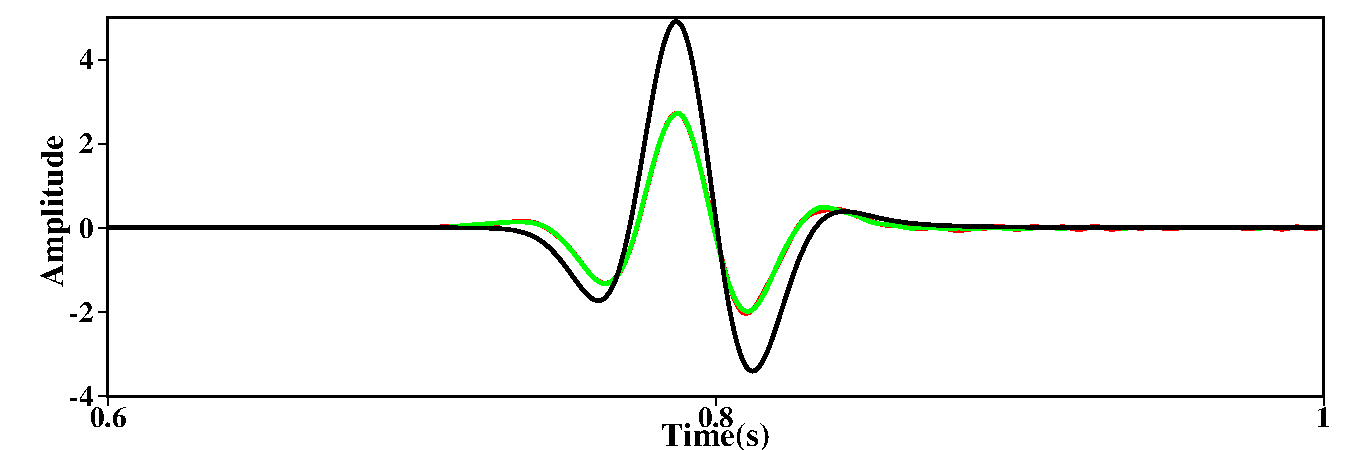
\includegraphics[width=0.8\textwidth]{Figure/chapter04/singlelayer/smooth3.pdf}}\\
   \subfloat[]{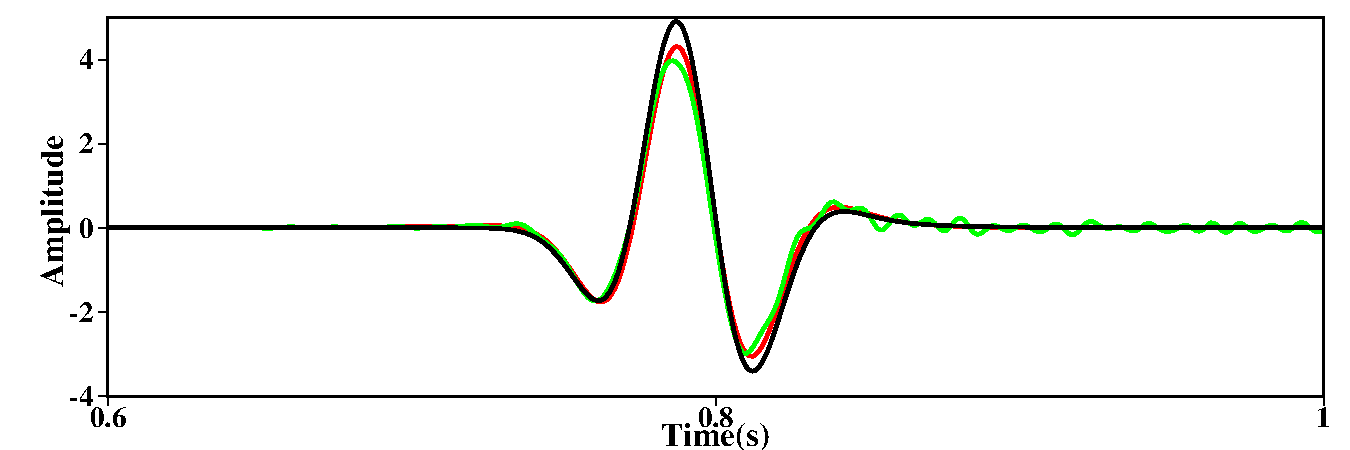
\includegraphics[width=0.8\textwidth]{Figure/chapter04/singlelayer/smooth8.pdf}}
   \caption{反射数据(黑)、反射数据与背景场的残差(红)和Born(绿)数据之间的差异。(a)
   模型平滑窗口30m; (b)模型平滑窗口100m.}
   \label{fig:refl_born_comparison}
\end{figure}
\begin{figure}[!htb]
   \centering
   \subfloat{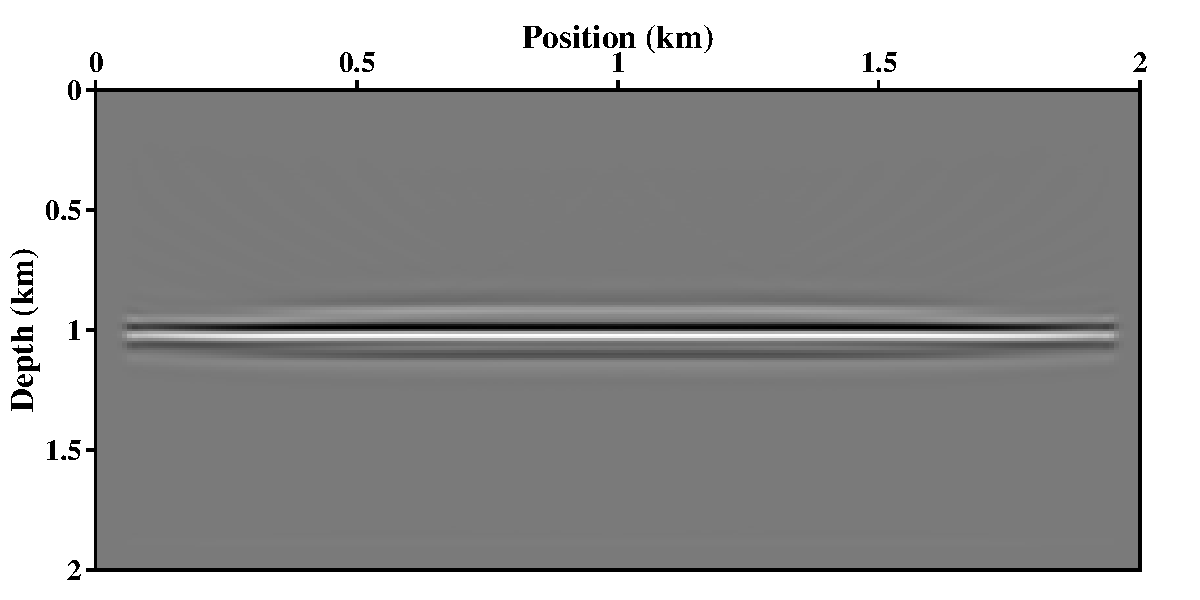
\includegraphics[width=0.5\textwidth]{Figure/chapter04/singlelayer/ref.pdf}
				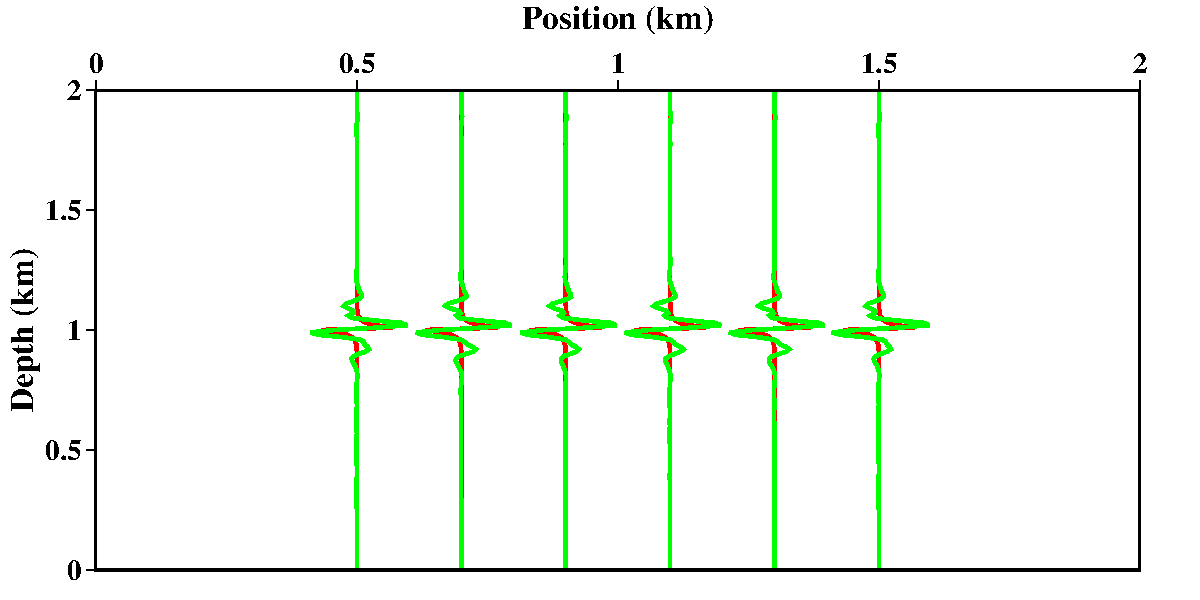
\includegraphics[width=0.5\textwidth]{Figure/chapter04/singlelayer/comparison1.pdf}}\\
   \subfloat{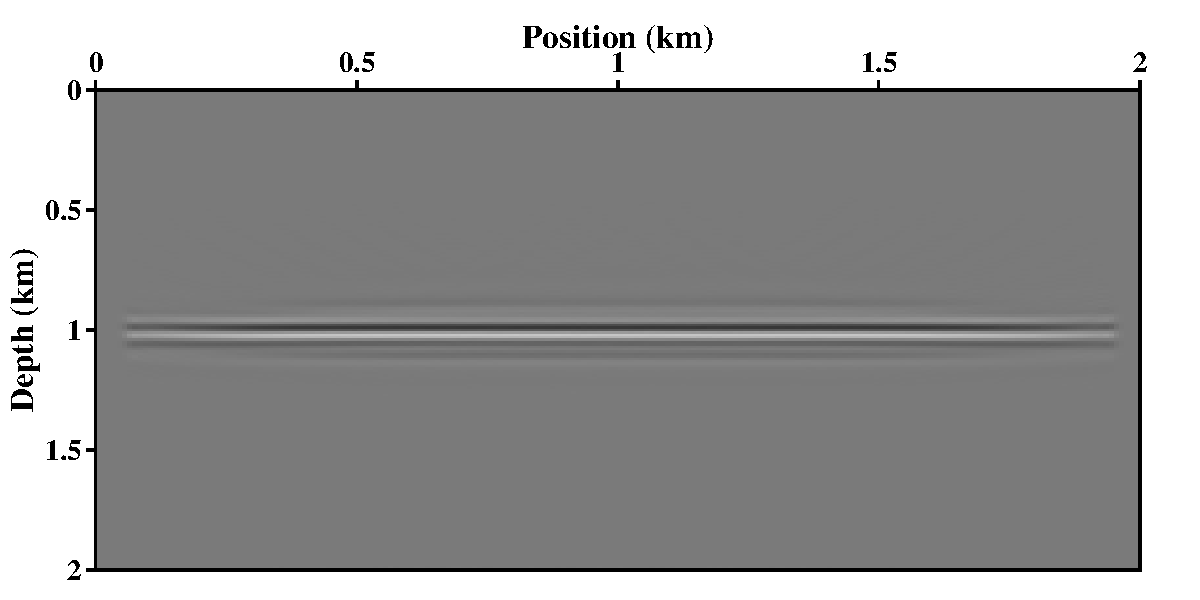
\includegraphics[width=0.5\textwidth]{Figure/chapter04/singlelayer/born.pdf}
			   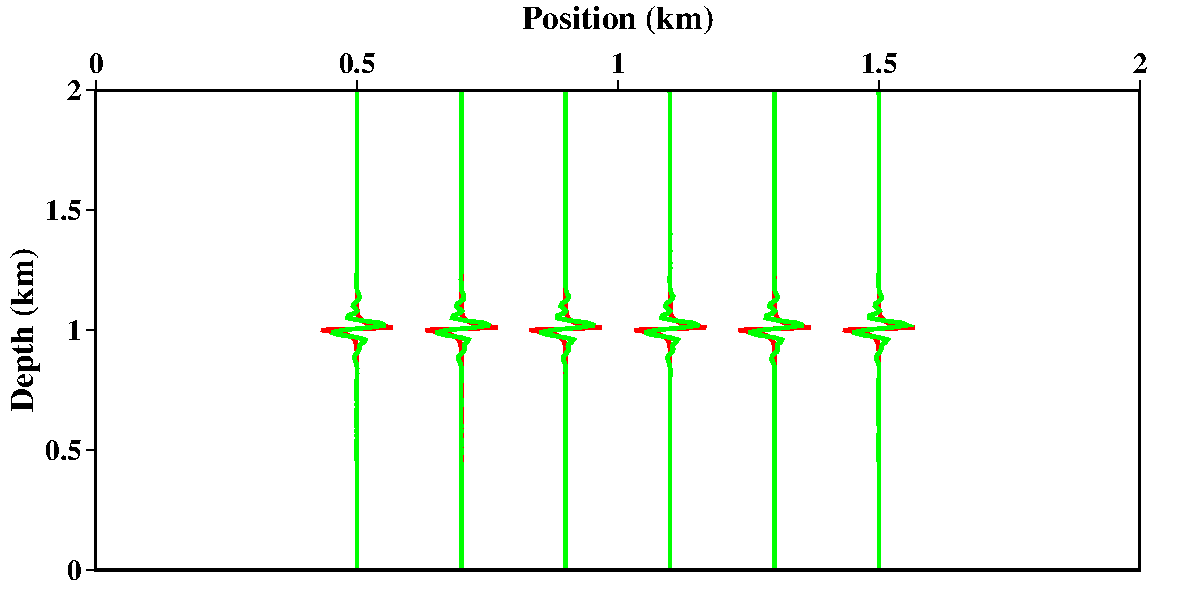
\includegraphics[width=0.5\textwidth]{Figure/chapter04/singlelayer/comparison2.pdf}}
%   \subfloat{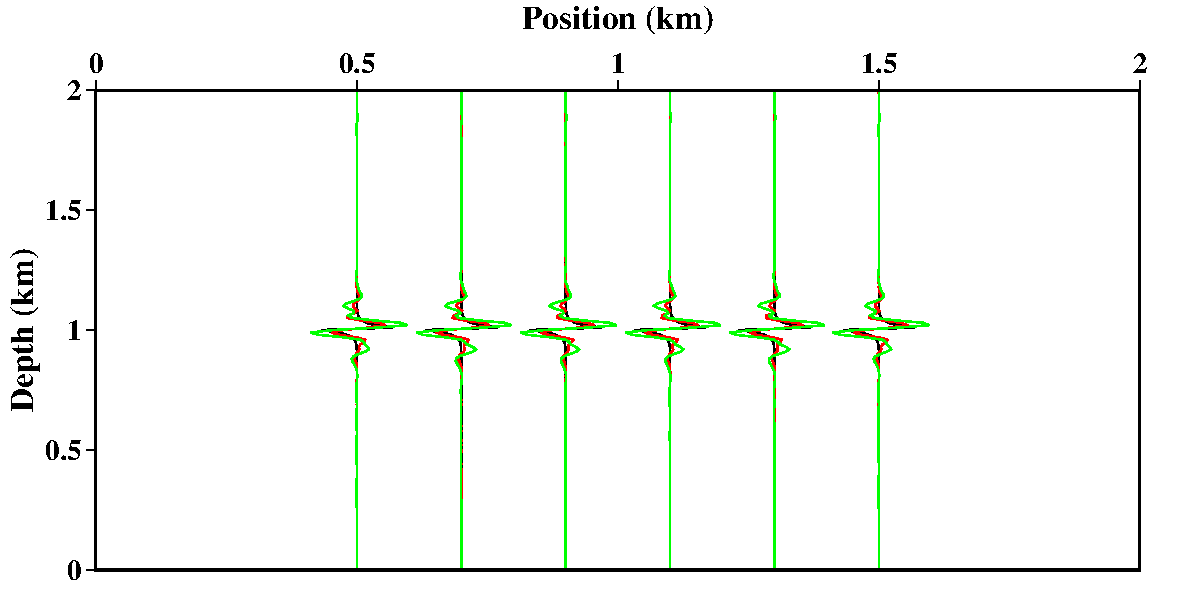
\includegraphics[width=0.5\textwidth]{Figure/chapter04/singlelayer/comparison.pdf}}
   \caption{图中左侧为E-LSRTM的$\delta
	   V_p$,右侧为相应位置上的抽线对比。顶部为反射残差数据反演结果,底部为Born数据反演结果。}
   \label{fig:Vpcomparison}
\end{figure}

图\ref{fig:refl_born_comparison}(a)所示为将真实模型按照30m半径平滑后所获得的反射数据、剩余反射数据(这里我们将
反射数据与背景波场记录的残差称为“剩余反射数据”)
以及真实扰动产生的Born数据之间的比较。可以看到当平滑半径较小时,背景模型中会包含部分高波数成分,这就使得背景场中产
生部分反射能量,从而导致Born数据会与真实反射数据相差较远。由于反射数据振幅大于真实Born数据的振幅,如果在反演中直接匹配该反射数据的振幅,
最终会导致在反演中数据残差收敛时产生参数扰动的过估计(图\ref{fig:Vpcomparison})。
但剩余反射数据可以与Born数据很好地匹配。

也就是说,如果模型中包含较强的反射能量,那么就需要匹配差异反射数据,而不是反射数据。
而如果模型平滑尺度较大,背景波场中包含的反射能量较弱,那么Born数据就不会与反射数据
相差太远,但即使如此,Born数据与反射数据之间的差异也大于其与剩余反射数据之间的差异
(图\ref{fig:refl_born_comparison}(b))。因此在LSRTM时,匹配剩余反射数据
将是一个更优的选择。
\subsection{参数耦合的影响}
参数耦合是E-LSRTM中面临的另一个挑战,E-LSRTM可以一定程度上消除参数间
彼此的干扰,例如Duan et al., 2016\cite{Duan2016},Feng and
Schuster,2016\cite{Feng2016}。但是他们也只能做到压制“脚印”,而难以完全消除,
尤其是在$V_p$与$V_s$结构不一致的时候。而模式解耦的梯度可以很好的帮助降低$V_s$反演中受到的参数耦合干扰。
为了测试参数耦合对E-LSRTM的影响以及模式解耦的有效性,我们选取具有不同结构的$V_p$与$V_s$双层模型来进行实验。
\begin{figure}[!htb]
   \centering
   \subfloat[]{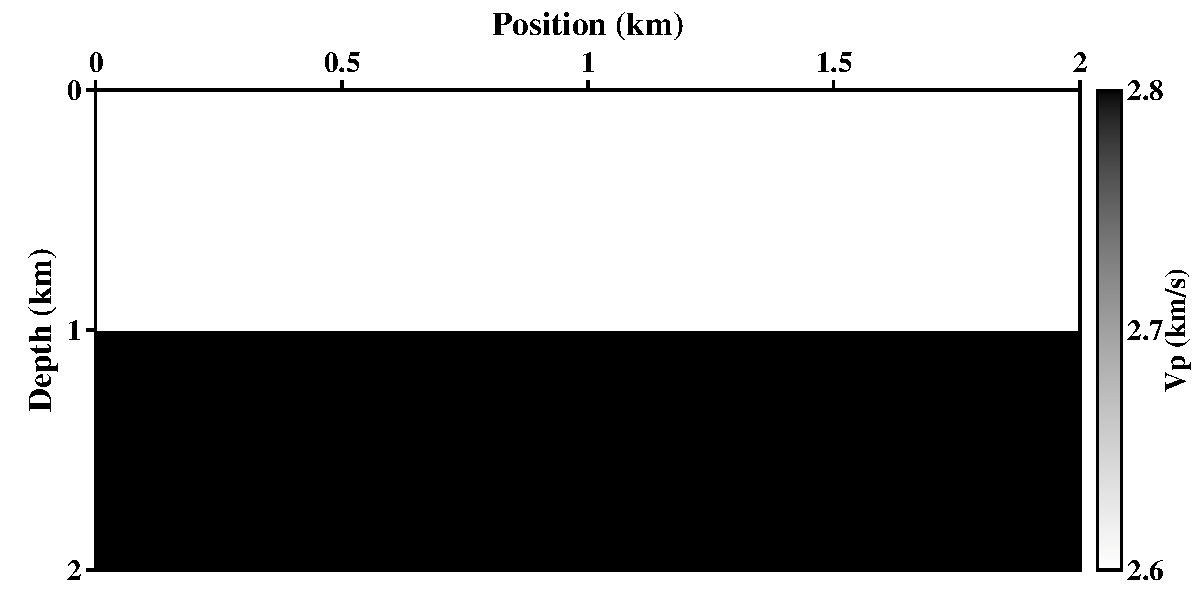
\includegraphics[width=0.5\textwidth]{Figure/chapter04/tradeoff/vp.pdf}}
   \subfloat[]{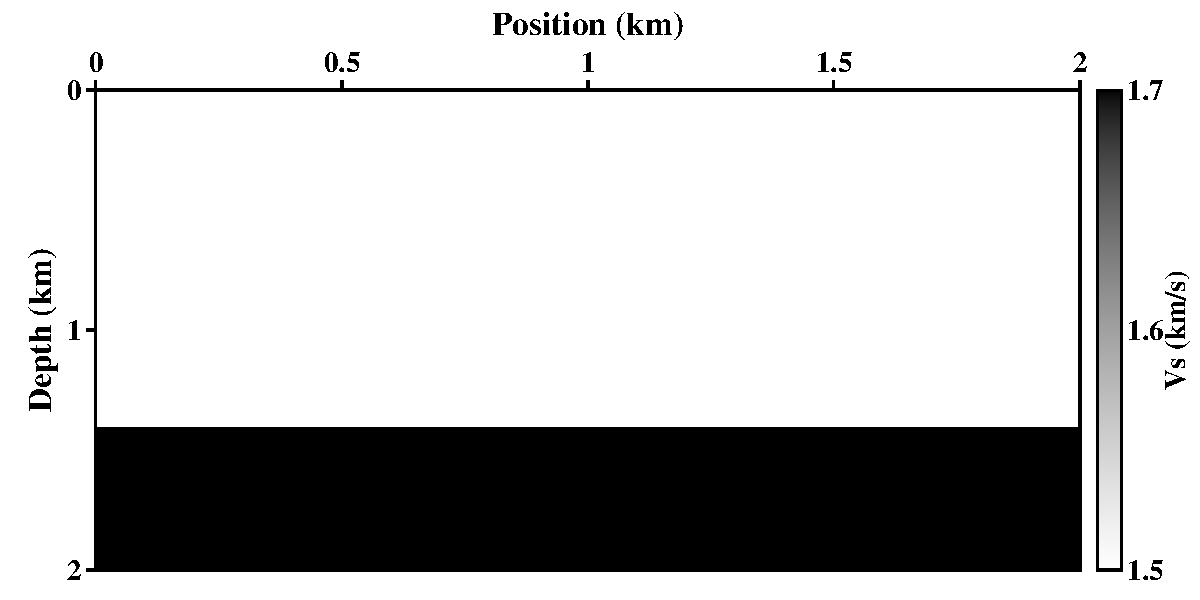
\includegraphics[width=0.5\textwidth]{Figure/chapter04/tradeoff/vs.pdf}}\\
   \caption{参数耦合测试真实模型,(a) $V_p$, (b) $V_s$.}
   \label{fig:tradeoffModel}
\end{figure}
\begin{figure}[!htb]
   \centering
   \subfloat[]{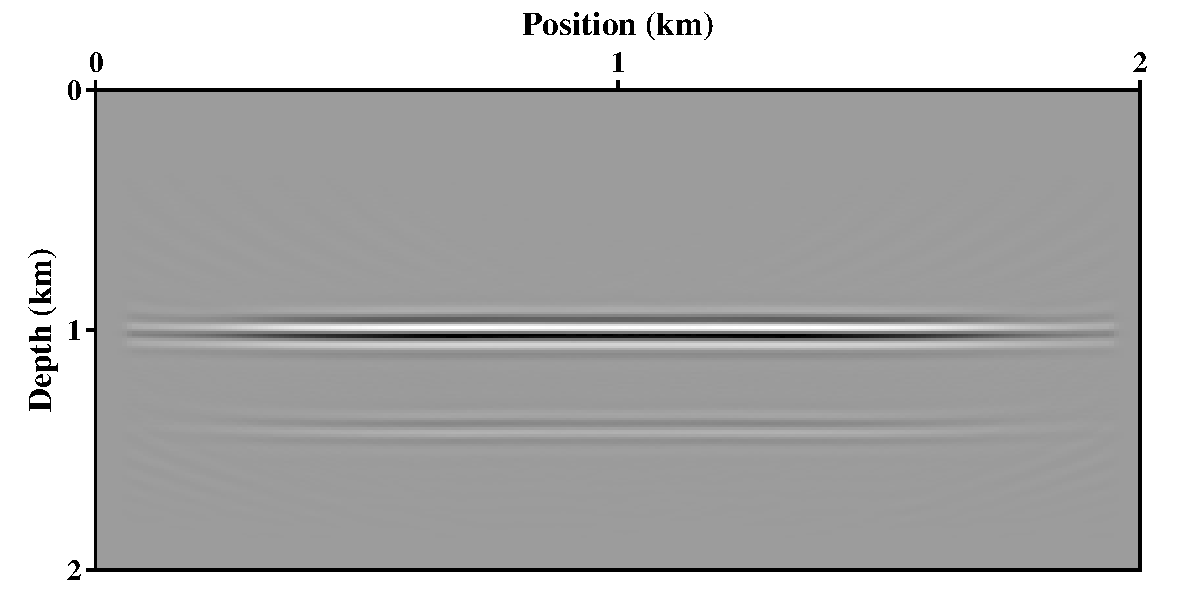
\includegraphics[width=0.5\textwidth]{Figure/chapter04/tradeoff/RTMvpnodecomp.pdf}}
   \subfloat[]{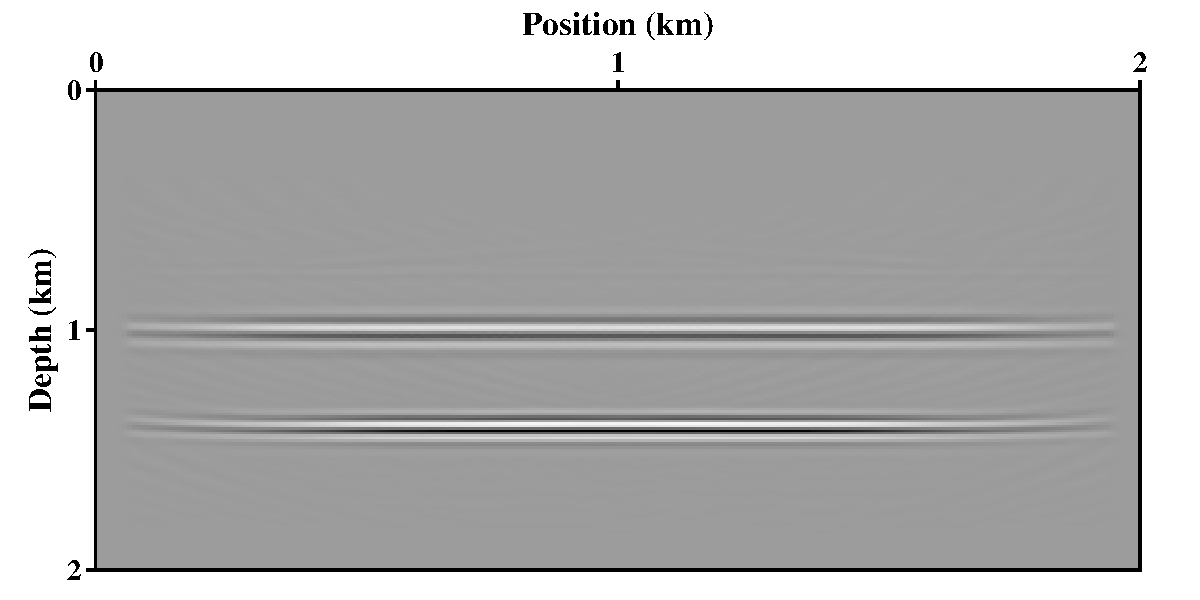
\includegraphics[width=0.5\textwidth]{Figure/chapter04/tradeoff/RTMvsnodecomp.pdf}}\\
   \subfloat[]{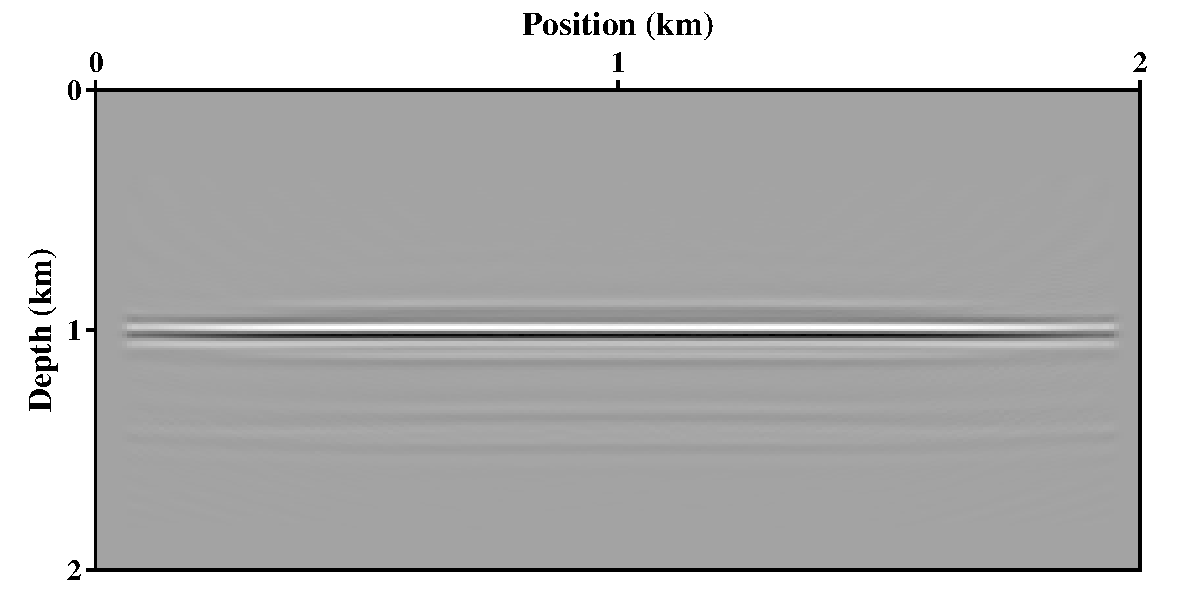
\includegraphics[width=0.5\textwidth]{Figure/chapter04/tradeoff/vpnodecomp.pdf}}
   \subfloat[]{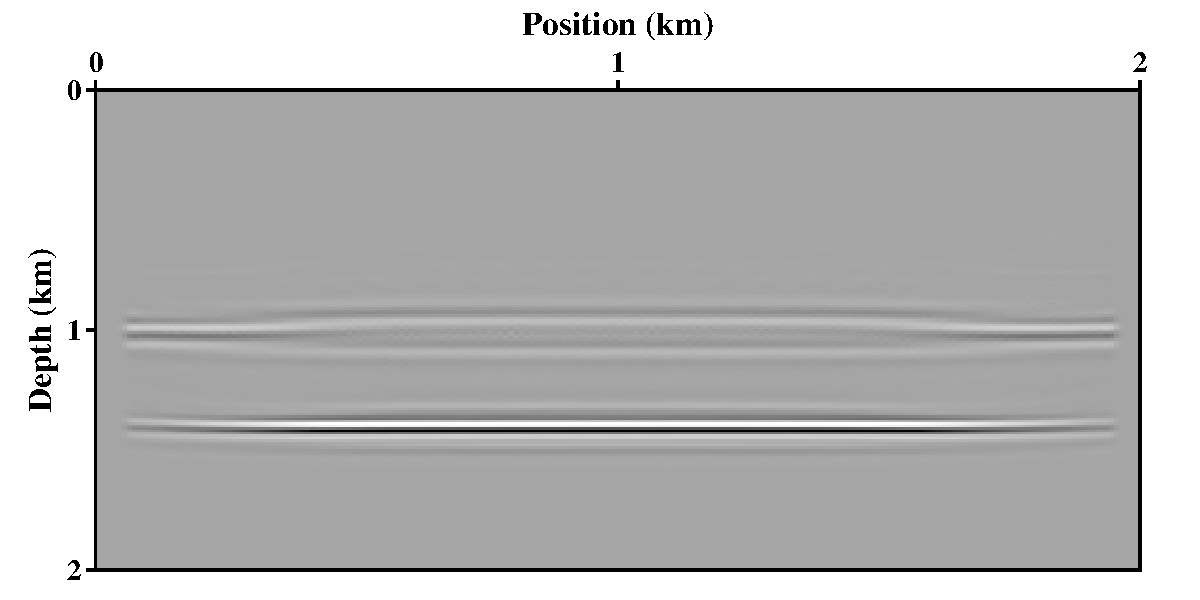
\includegraphics[width=0.5\textwidth]{Figure/chapter04/tradeoff/vsnodecomp.pdf}}
   \caption{常规ERTM与E-LSRTM结果。左侧为$\delta V_p$,右侧为$\delta V_s$。(a), (b)为ERTM结果,(c),
   (d)为E-LSRTM结果。}
   \label{fig:tradeoff_nodecomp}
\end{figure}
\begin{figure}[!htb]
   \centering
   \subfloat[]{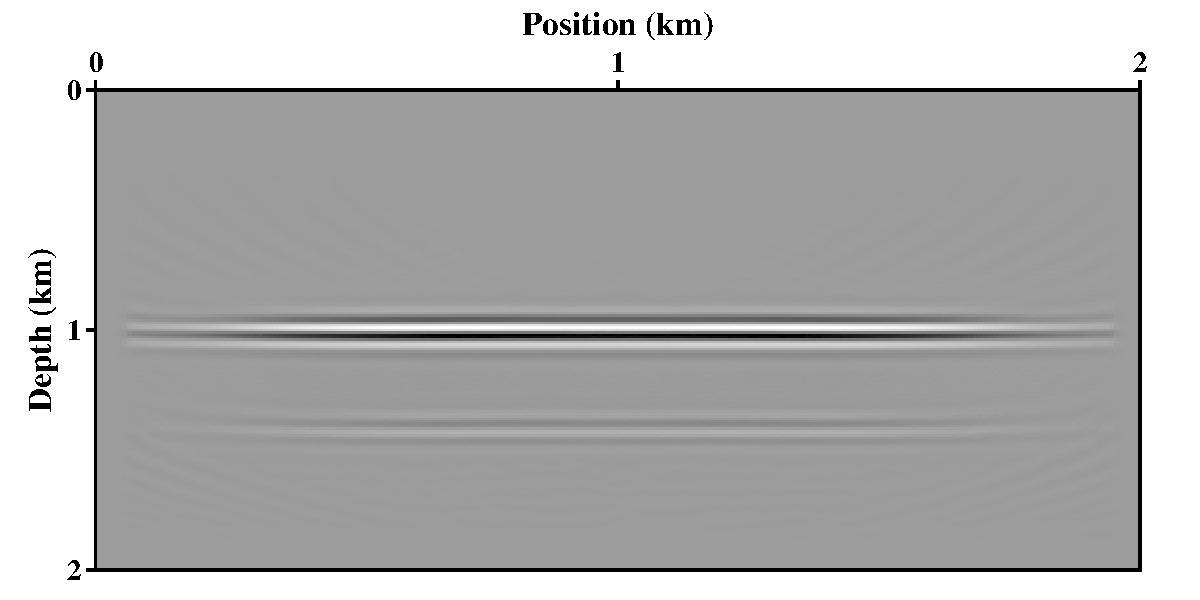
\includegraphics[width=0.5\textwidth]{Figure/chapter04/tradeoff/RTMvpdecomp.pdf}}
   \subfloat[]{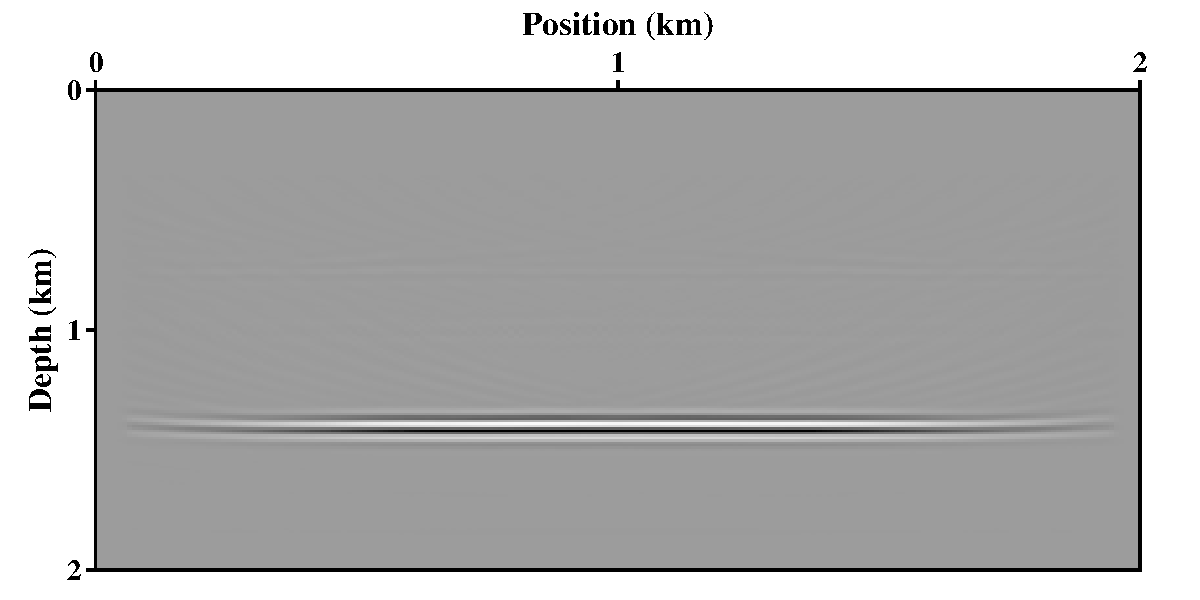
\includegraphics[width=0.5\textwidth]{Figure/chapter04/tradeoff/RTMvsdecomp.pdf}}\\
   \subfloat[]{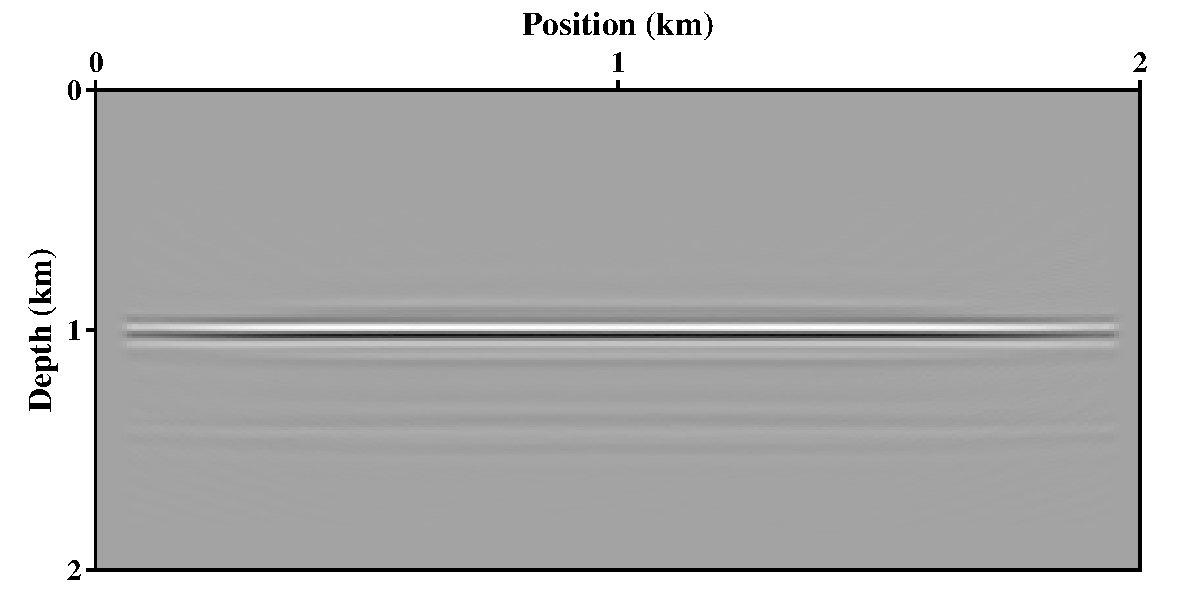
\includegraphics[width=0.5\textwidth]{Figure/chapter04/tradeoff/vpdecomp.pdf}}
   \subfloat[]{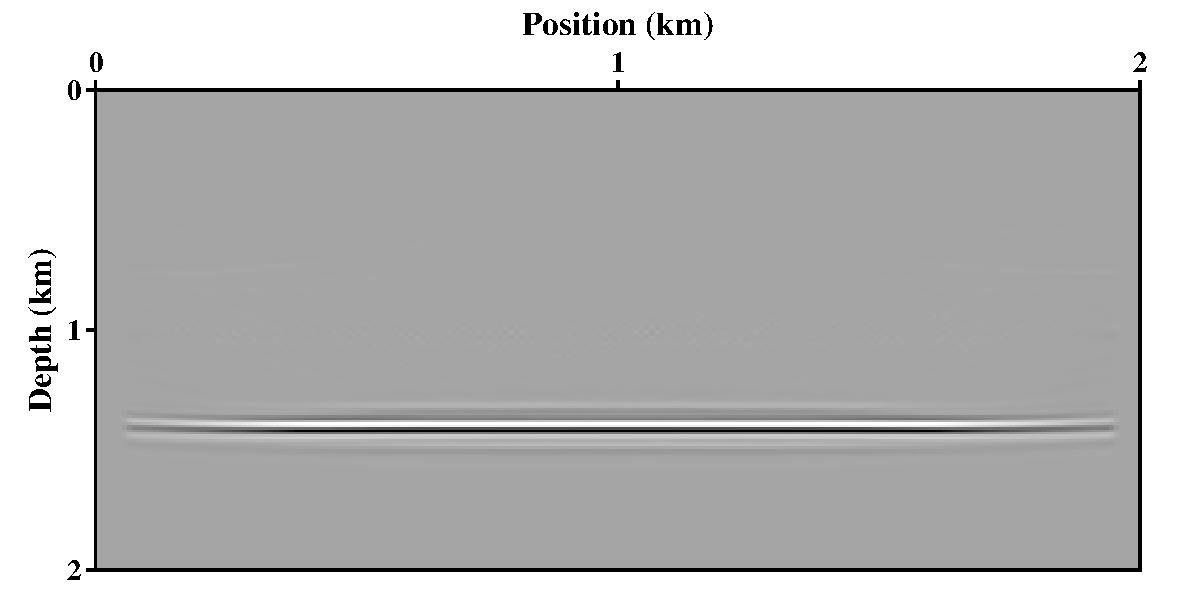
\includegraphics[width=0.5\textwidth]{Figure/chapter04/tradeoff/vsdecomp.pdf}}\\
   \subfloat[]{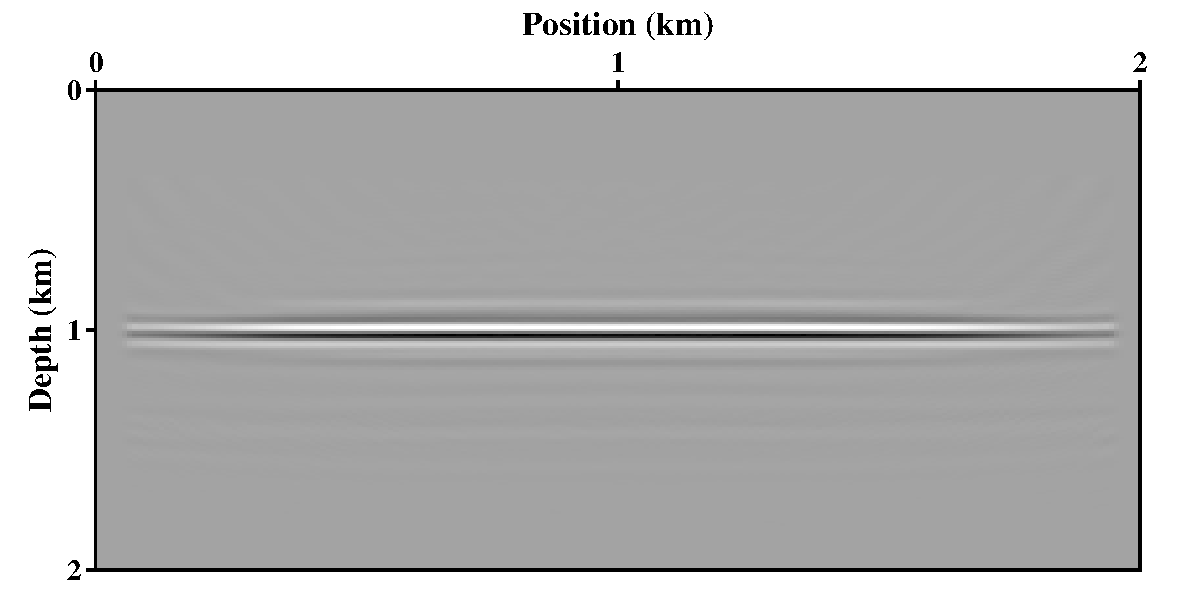
\includegraphics[width=0.5\textwidth]{Figure/chapter04/tradeoff/2ndvpdecomp.pdf}}
   \subfloat[]{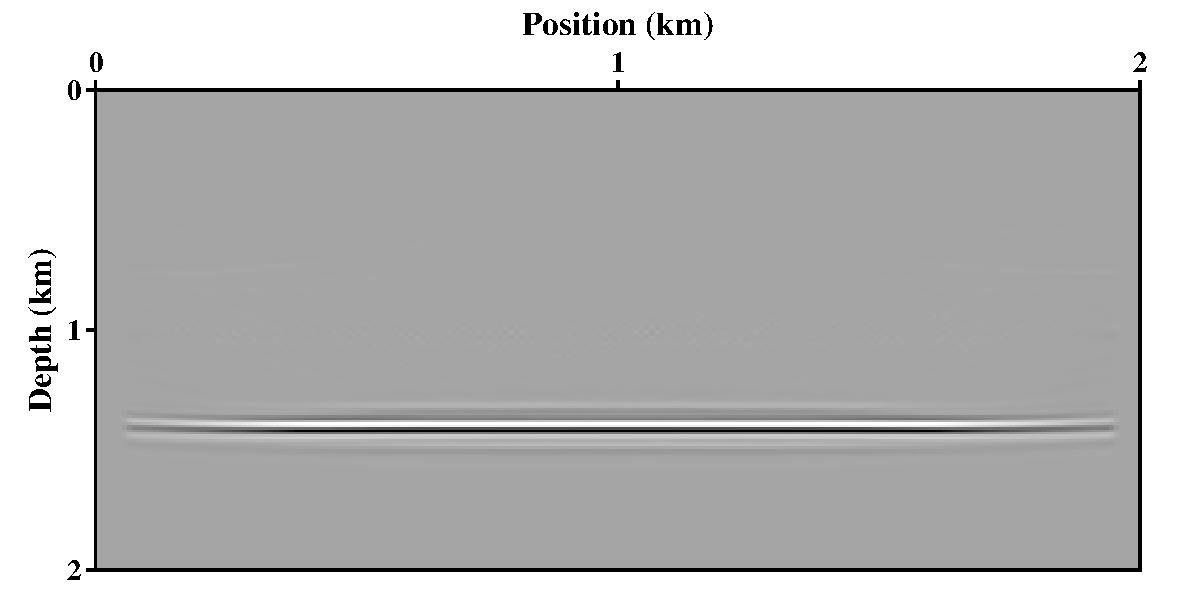
\includegraphics[width=0.5\textwidth]{Figure/chapter04/tradeoff/vsdecomp.pdf}}
   \caption{模式解耦预条件的ERTM与E-LSRTM结果。左侧为$\delta V_p$,右侧为$\delta V_s$。(a),
   (b)为ERTM结果; (c), (d)为采用策略1时E-LSRTM结果;(e), (f)为采用策略2时E-LSRTM结果。}
   \label{fig:tradeoff_decomp}
\end{figure}

真实模型如图\ref{fig:tradeoffModel}所示。这里我们采用Born正演数据进行双参数同时反演。
由于$V_s$界面也会产生P波反射,因此如图\ref{fig:tradeoff_nodecomp}中,
常规RTM结果中$V_p$与$V_s$成像结果中存在明显的相互影响,而E-LSRTM过程可以消除部分参数耦合的效应,
但是难以完全压制,尤其是$\delta V_s$中存在非常明显的$\delta V_p$脚印。

而加入模式解耦之后,
我们首先采用策略1进行反演。
由于采用S波波场来计算$\delta V_s$梯度,
这就可以完全避免了P波对$\delta
V_s$梯度的干扰效应。根据第二章中所分析的模式解耦帮助压制参数耦合的机制,采用S波反演$V_s$近似于单参数反演,这将
有助于$V_s$的收敛。但是对于$\delta
V_p$的反演提升没有这么明显,只能依靠在迭代过程中$\delta
V_s$趋近于真值时来消除其所产生的P波数据残差,进而提升$\delta V_p$的反演效果。

从ERTM结果上看,解耦之后的成像结果已经可以压制$\delta V_s$中
$V_p$界面产生的脚印。而解耦预条件的E-LSRTM得到的$\delta
V_s$已经没有了$V_p$界面的脚印干扰,但是$\delta
V_p$中仍然存在一定的干扰,这是因为在策略1中,初始迭代阶段时$\delta
V_s$反演更新量不足,使得$\delta
V_p$的梯度总是存在脚印的影响,而在此阶段中总是能够搜索到较大的更新步长,这就导致在初始阶段的参数耦合效应仍然较为严重。而且主要是
$\delta V_p$受到$\delta V_s$的影响。
策略2可以进一步压制这种类型的干扰,在$\delta
V_s$反演足够好的时候$V_s$界面产生的P波数据已经基本匹配,这时再反演$\delta
V_p$就能够最小化$V_s$界面在$\delta V_p$中的影响。
然而反演得到的$\delta V_s$不可能与真值一样,这样数据残差中就一定存在少量的来自$\delta
V_s$的P波。因此可以看到即使采用策略2,$\delta V_p$中最终还会存留非常弱的脚印。


\subsection{Marmousi模型}
本节将在Marmousi模型上进行算法的测试,为了降低计算代价,$V_s$模型通过固定的泊凇比获得。
观测系统中,60个炮点等间隔地分布在地表,为了提高成像质量检波点被置放在第一个反射界面附近。模型空间采样间隔
为10m,时间采样间隔为1ms,模拟时间总长3s,子波主频20Hz。除非特别指明,本节中所有数值实验都采用上述相同的观测系统。
为了对比Born数据与反射残差数据间的反演差异,
每个模型都采用Born数据与反射残差数据各进行一次E-LSRTM。
\begin{figure}[!htb]
   \centering
   \subfloat[]{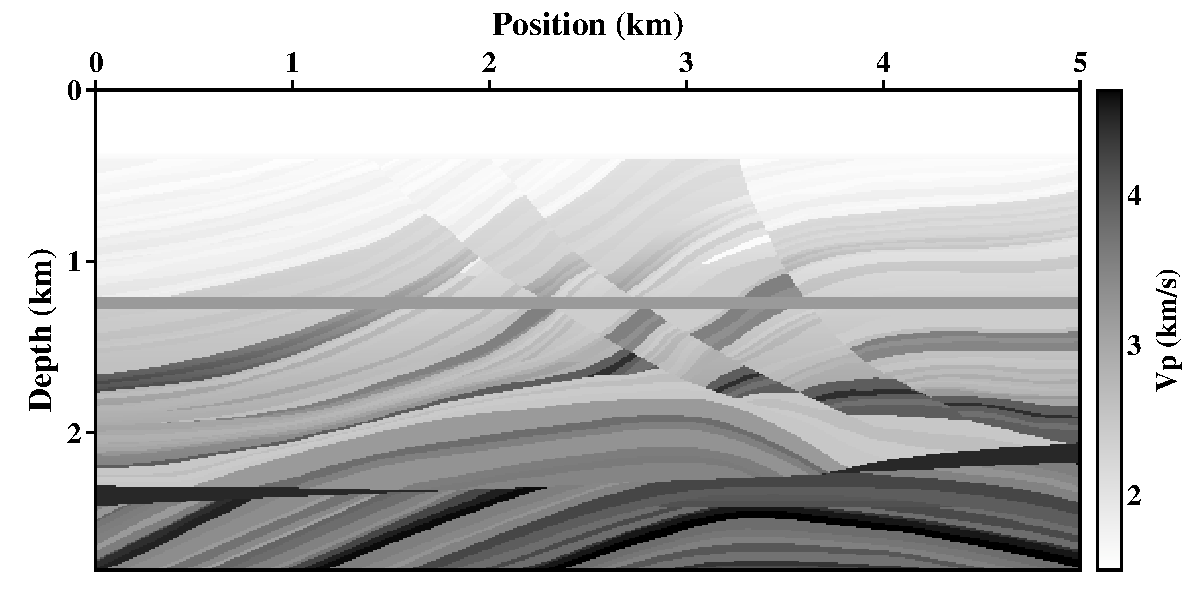
\includegraphics[width=0.5\textwidth]{Figure/chapter04/Marmousi/born/vp.pdf}}
   \subfloat[]{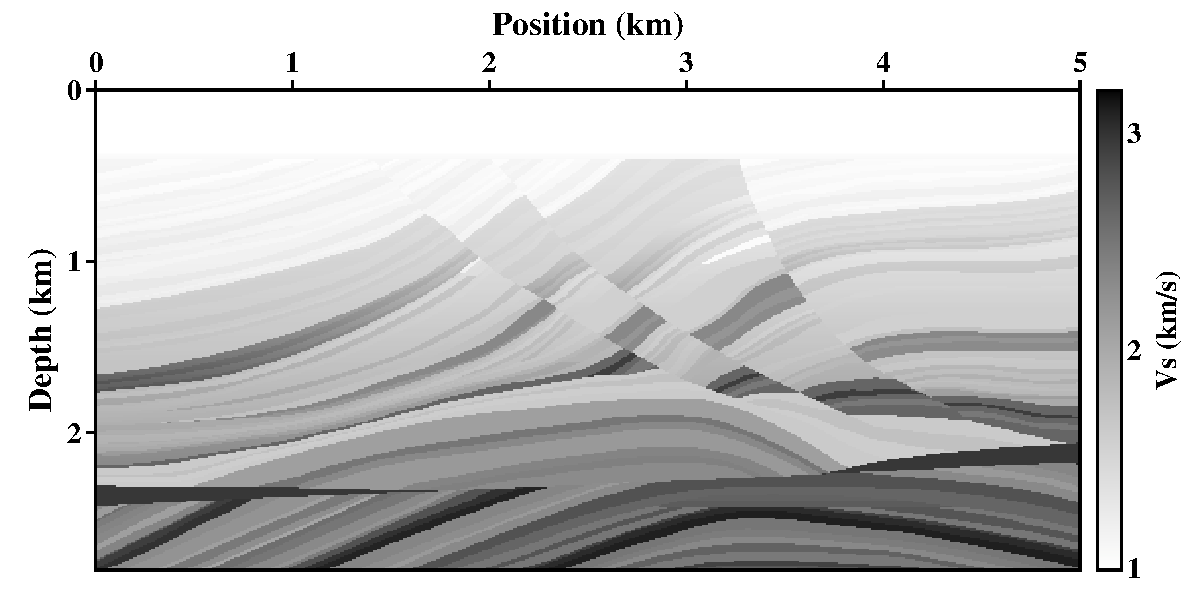
\includegraphics[width=0.5\textwidth]{Figure/chapter04/Marmousi/born/vs.pdf}}\\
   \subfloat[]{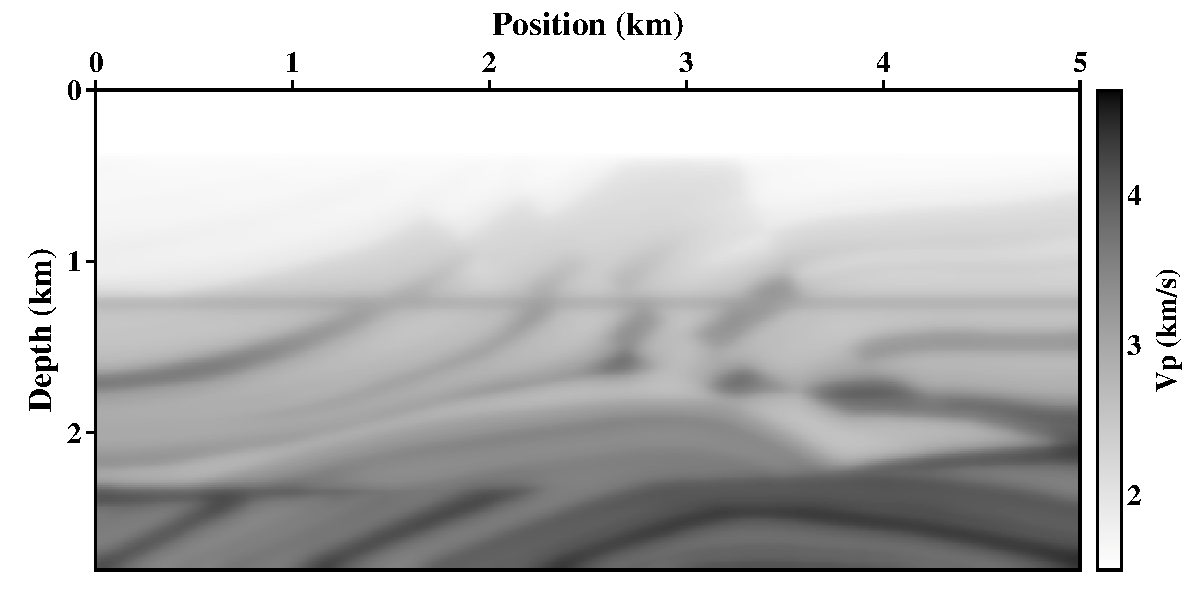
\includegraphics[width=0.5\textwidth]{Figure/chapter04/Marmousi/born/vpsmooth.pdf}}
   \subfloat[]{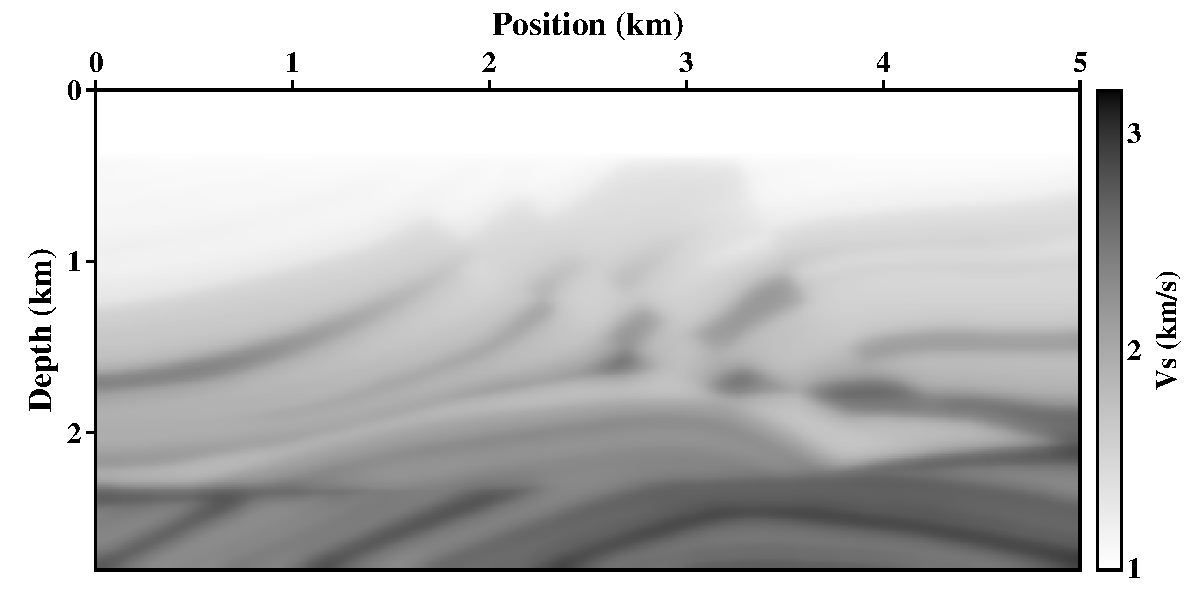
\includegraphics[width=0.5\textwidth]{Figure/chapter04/Marmousi/born/vssmooth.pdf}}
   \caption{Marmousi真实模型与偏移模型。左侧为$V_p$,右侧为$V_s$。第一行为真实模型,第二行为偏移模型。}
   \label{fig:TrueAndInitial_1}
\end{figure}
\begin{figure}[!htb]
   \centering
   \subfloat[]{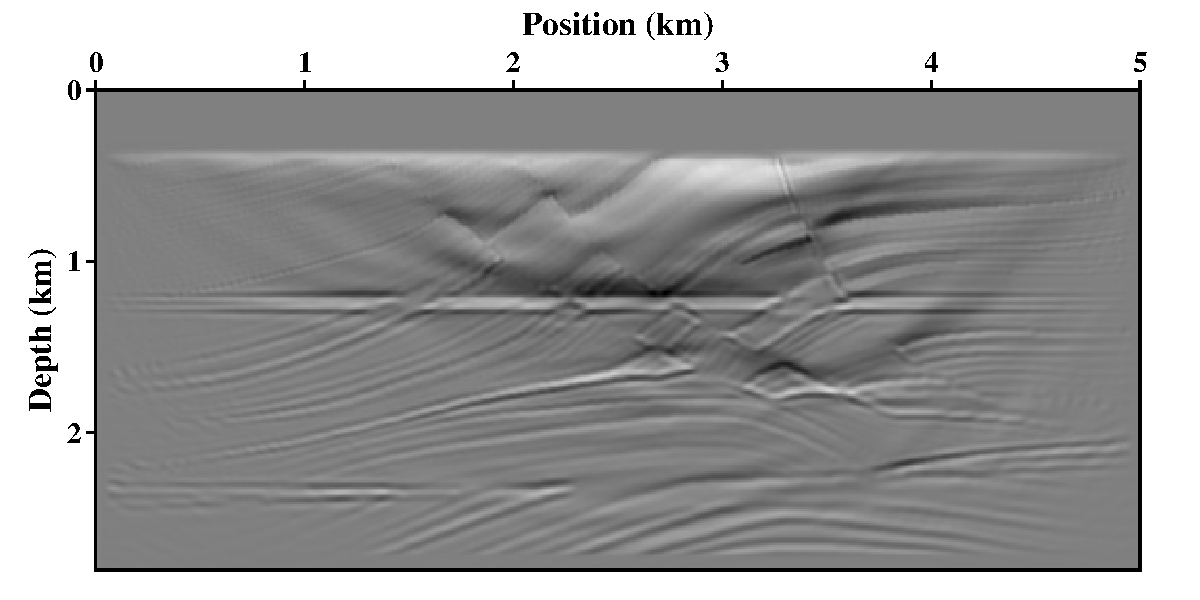
\includegraphics[width=0.5\textwidth]{Figure/chapter04/Marmousi/born/RTMvpnodecomp.pdf}}
   \subfloat[]{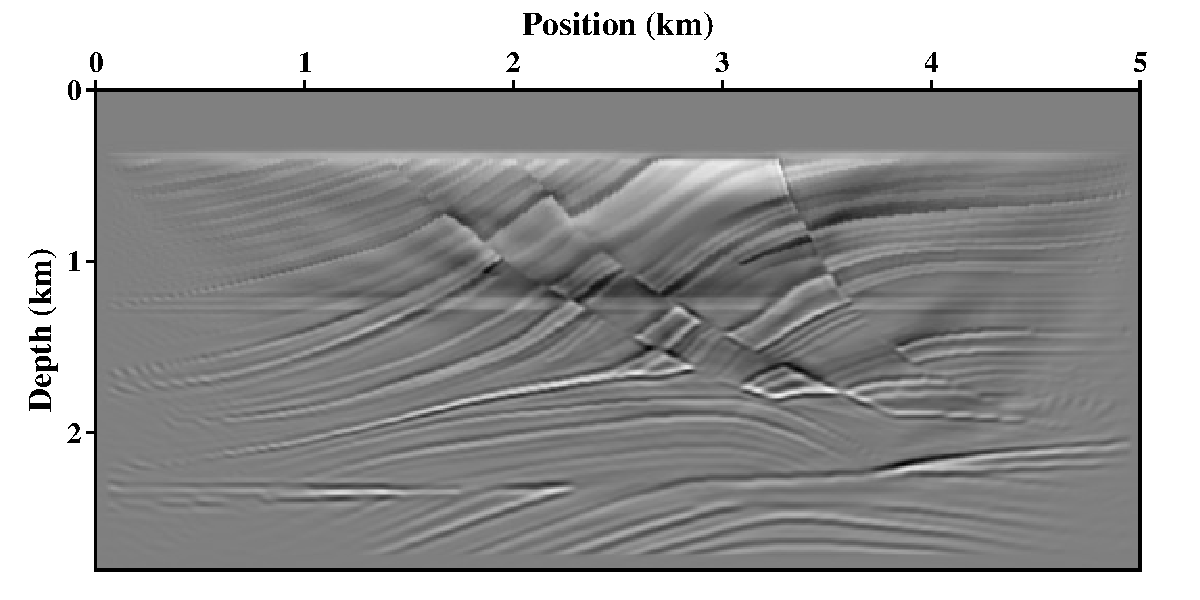
\includegraphics[width=0.5\textwidth]{Figure/chapter04/Marmousi/born/RTMvsnodecomp.pdf}}\\
   \subfloat[]{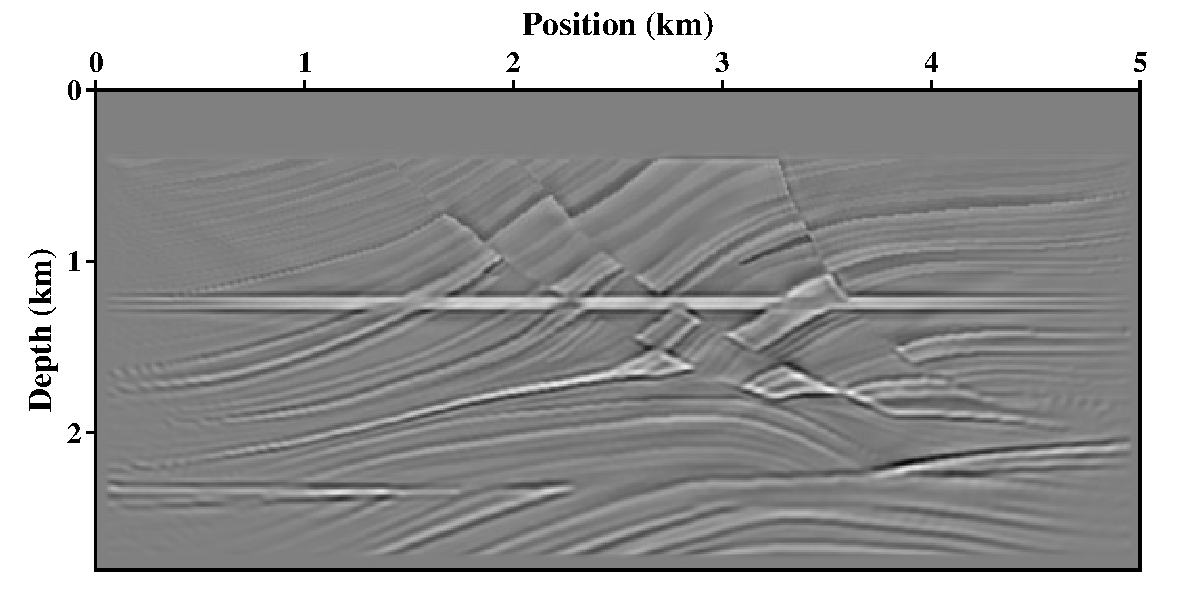
\includegraphics[width=0.5\textwidth]{Figure/chapter04/Marmousi/born/vpnodecomp.pdf}}
   \subfloat[]{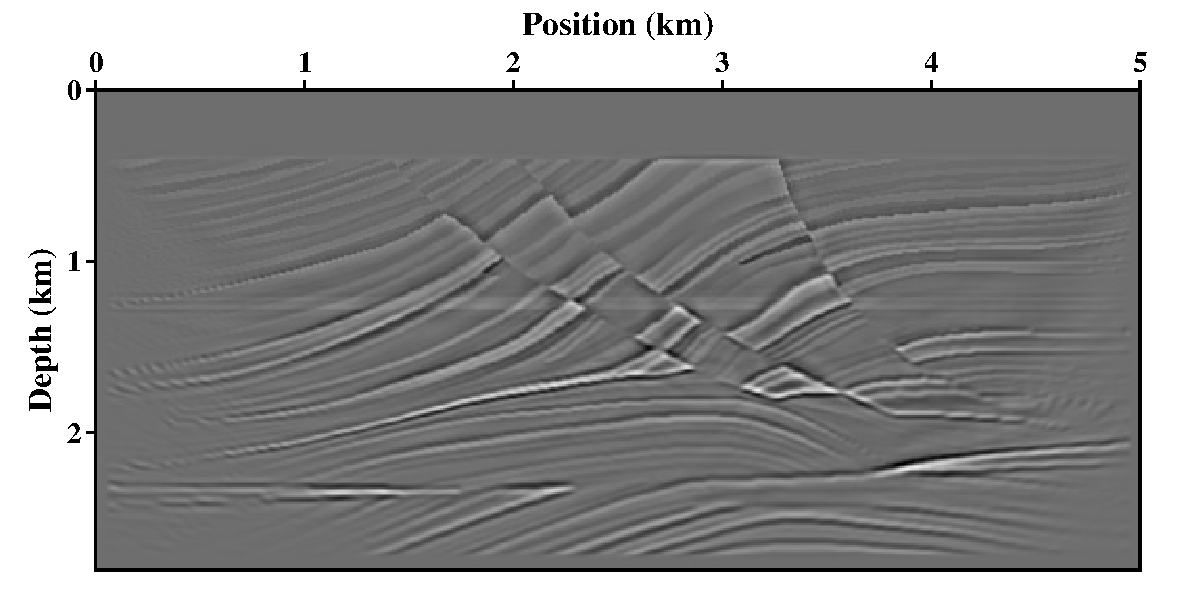
\includegraphics[width=0.5\textwidth]{Figure/chapter04/Marmousi/born/vsnodecomp.pdf}}
   \caption{Born数据常规ERTM与E-LSRTM结果。左侧为$V_p$,右侧为$V_s$。第一行为ERTM结果,第二行为E-LSRTM结果。}
   \label{fig:nodecomp_1}
\end{figure}
\begin{figure}[!htb]
   \centering
   \subfloat[]{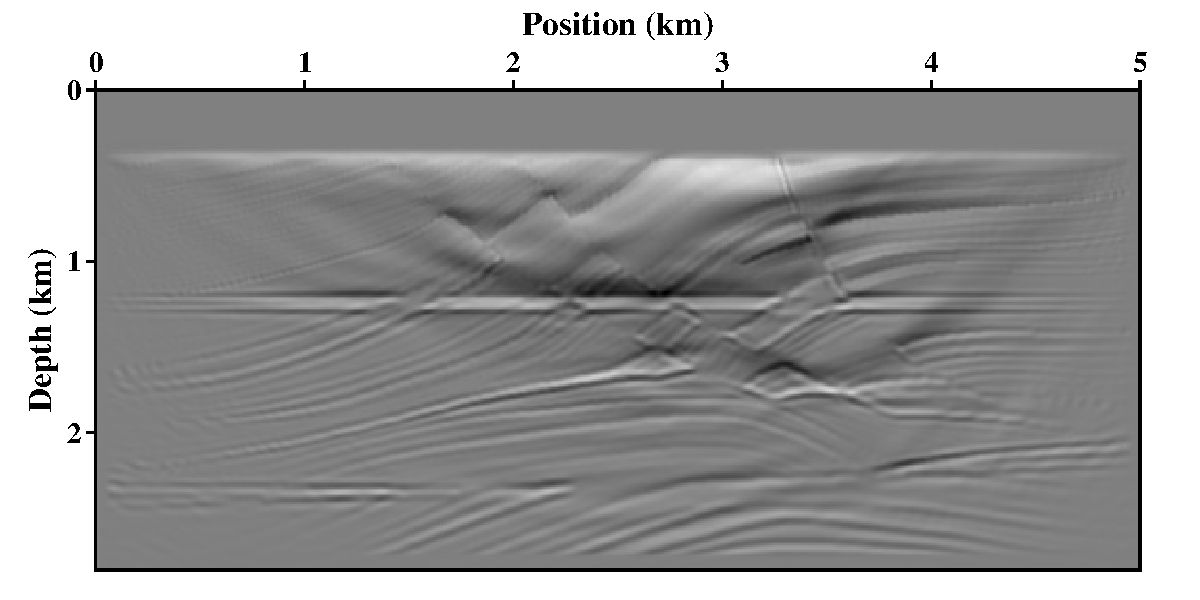
\includegraphics[width=0.5\textwidth]{Figure/chapter04/Marmousi/born/RTMvpdecomp.pdf}}
   \subfloat[]{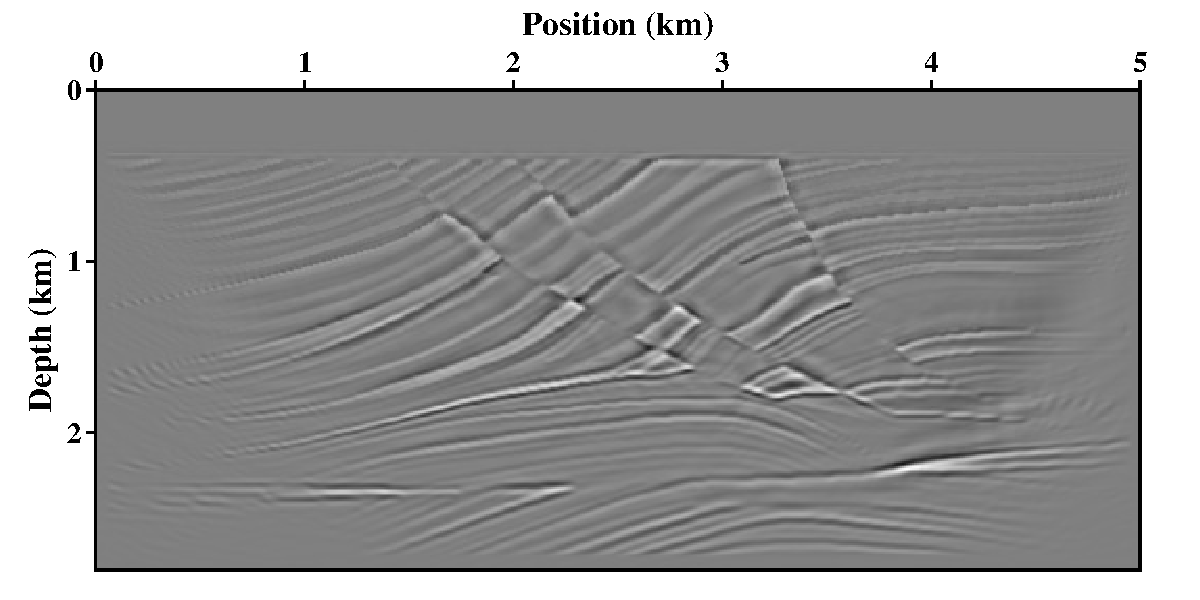
\includegraphics[width=0.5\textwidth]{Figure/chapter04/Marmousi/born/RTMvsdecomp.pdf}}\\
   \subfloat[]{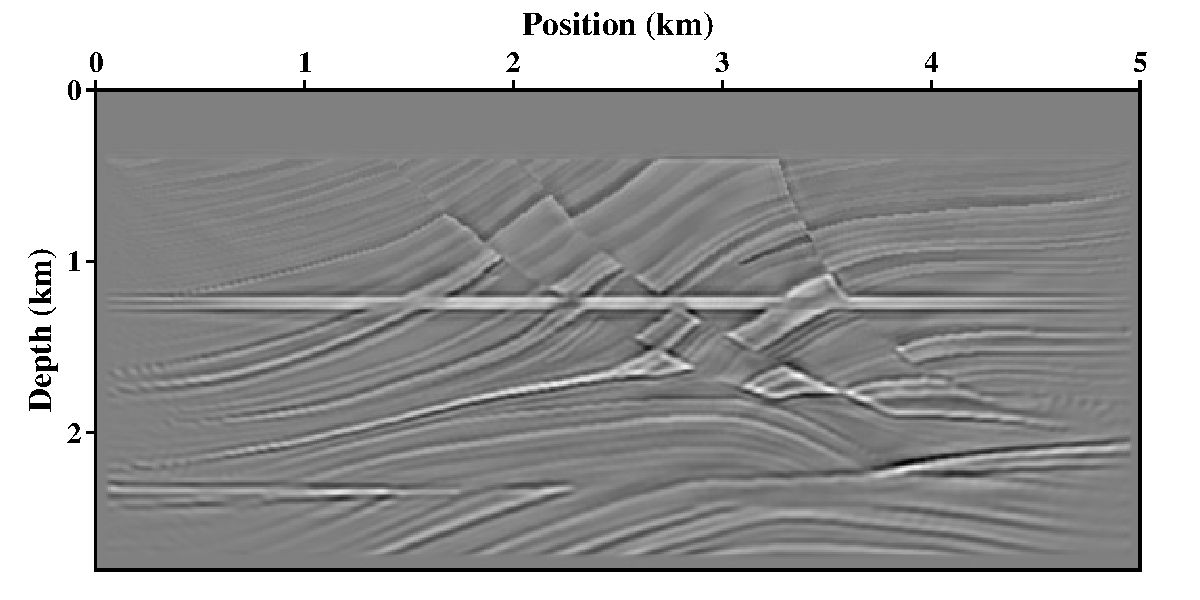
\includegraphics[width=0.5\textwidth]{Figure/chapter04/Marmousi/born/vpdecomp.pdf}}
   \subfloat[]{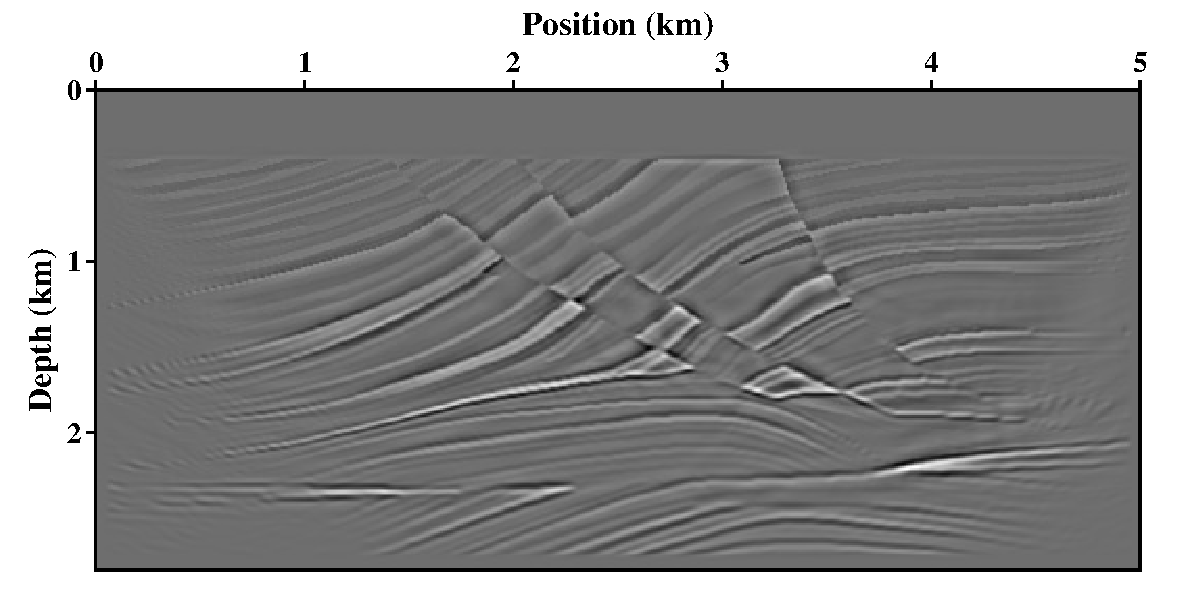
\includegraphics[width=0.5\textwidth]{Figure/chapter04/Marmousi/born/vsdecomp.pdf}}\\
   \caption{Born数据模式解耦下ERTM与E-LSRTM结果。左侧为$V_p$,右侧为$V_s$。第一行为ERTM结果,第二行为E-LSRTM结果。}
   \label{fig:decomp_1}
\end{figure}

第一个实验中,为了突出参数耦合效应,在$V_p$模型中加入了一个高速薄层。这样在常规E-LSRTM中,$\delta
V_s$的反演会受到参数耦合的干扰,由于$\delta V_p$中则较少受到$V_s$结构的影响,因此可以采用反演策略1,同时反演$\delta
V_p$与$\delta V_s$。首先我们采用Born数据进行E-LSRTM。如图\ref{fig:nodecomp_1}所示,常规ERTM结果中,$V_p$和$V_s$成像中
可以看到低频噪音的干扰,并且由于参数耦合,$\delta
V_s$中还存在$V_p$结构的影子。在经过E-LSRTM之后,低频噪音被压制,
整个成像剖面能量更加均衡
而且$V_s$中的参数耦合干扰也被部分消除了,但是仍然可以明显的看到残留的干扰脚印。

之后将模式解耦的预条件加入到梯度计算中,结果如图\ref{fig:decomp_1}所示,ERTM结果中$\delta
V_p$仍然存在低频噪音,而$\delta
V_s$中的低频噪音已经很少了,这说明低频噪音主要是PP波路径所产生,在经过解耦之后,反传P波被压制,所以$\delta
V_s$中基本消除了低频噪音。而且ERTM结果中也可以看到来自$V_p$结构的脚印已经被完全压制掉了。在经过E-LSRTM之后,采用解耦预条件的方法获得了
很好的$\delta V_p$与$\delta V_s$的反演结果。
\begin{figure}[!htb]
   \centering
   \subfloat[]{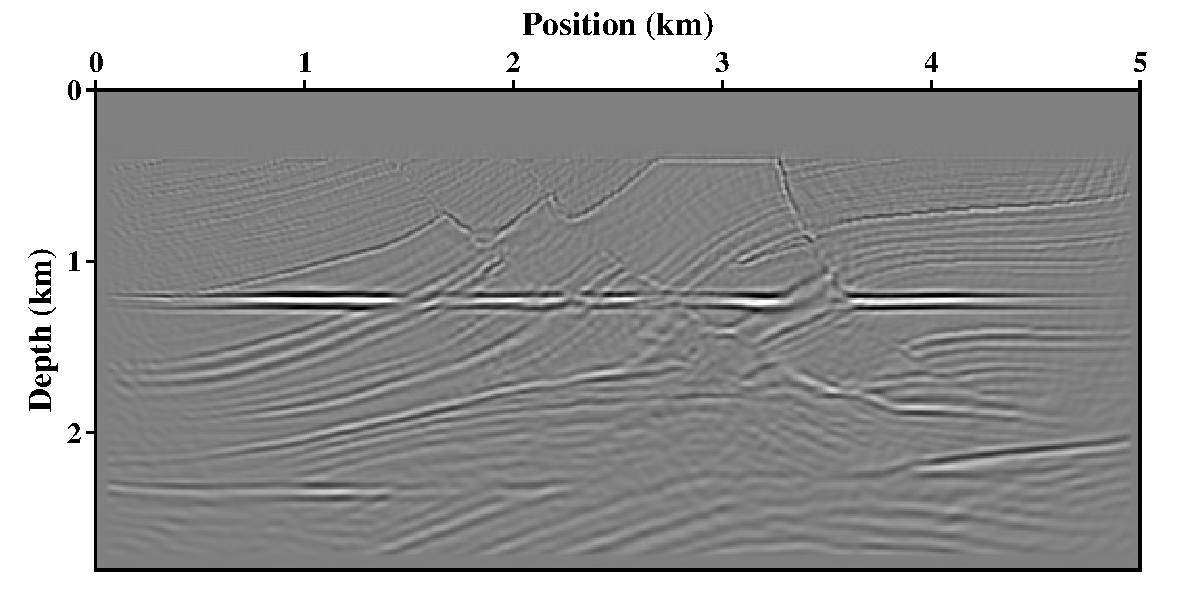
\includegraphics[width=0.5\textwidth]{Figure/chapter04/Marmousi/reflection/RTMvpnodecomp.pdf}}
   \subfloat[]{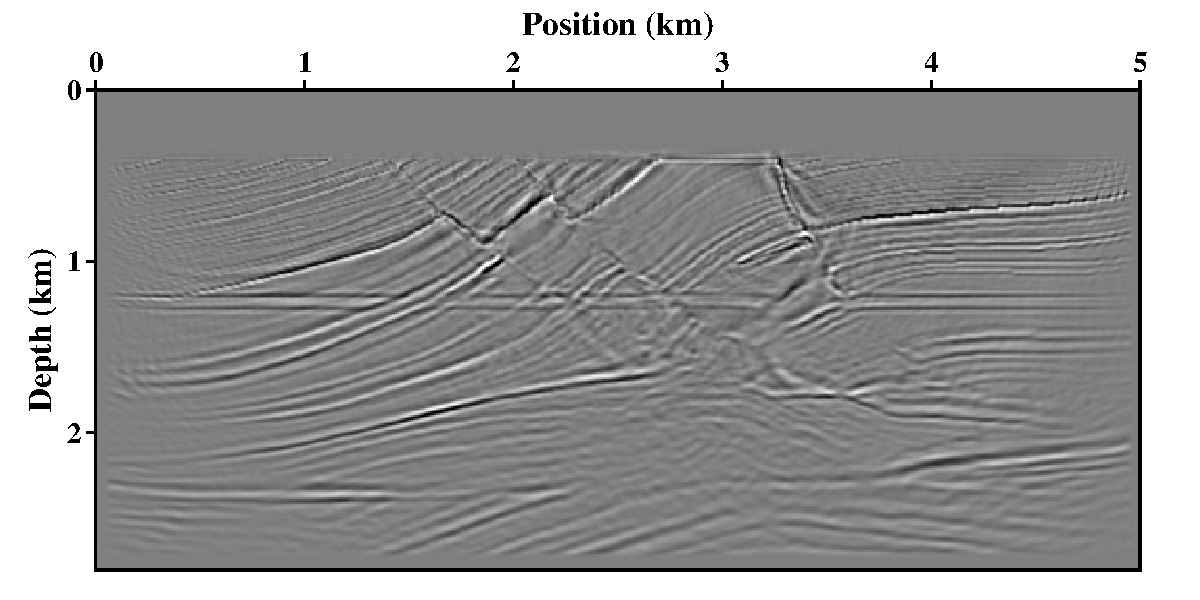
\includegraphics[width=0.5\textwidth]{Figure/chapter04/Marmousi/reflection/RTMvsnodecomp.pdf}}\\
   \subfloat[]{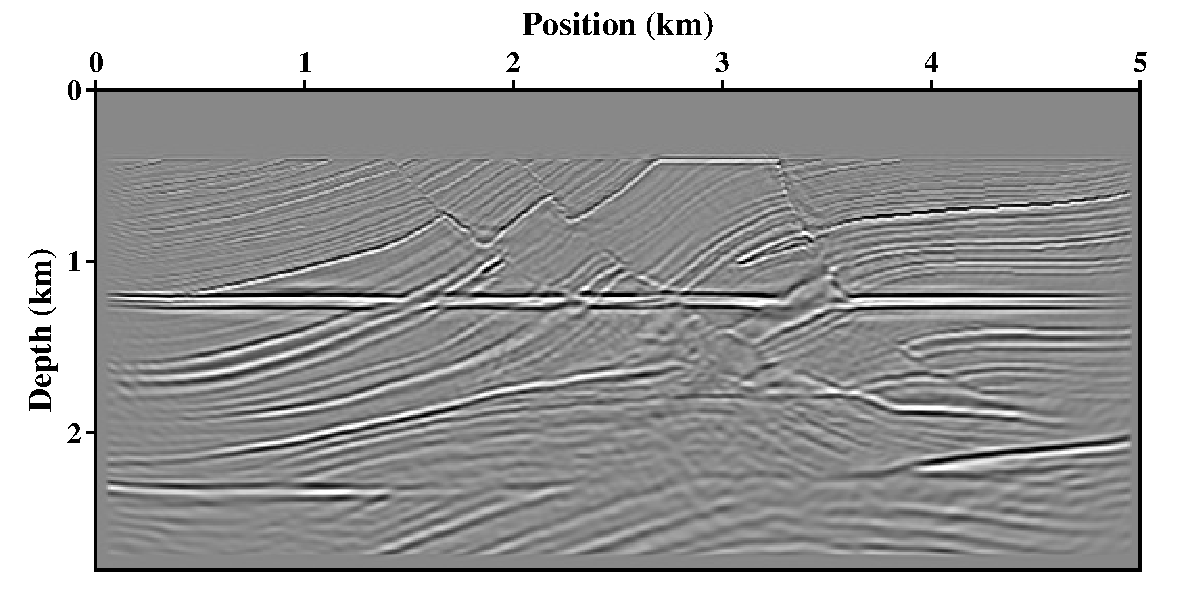
\includegraphics[width=0.5\textwidth]{Figure/chapter04/Marmousi/reflection/vpnodecomp.pdf}}
   \subfloat[]{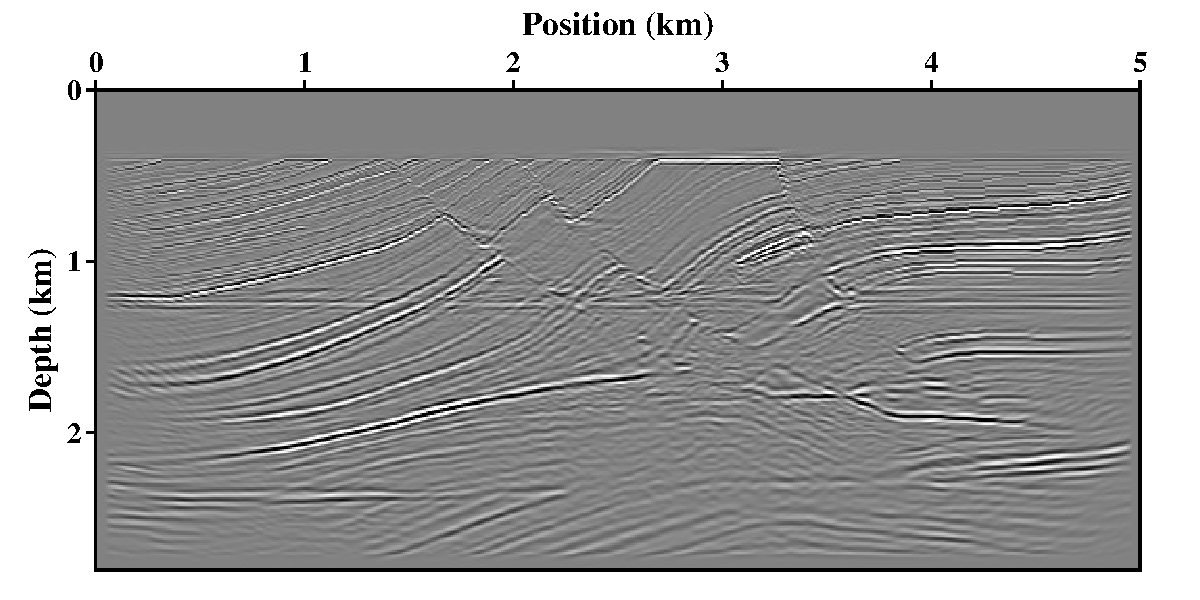
\includegraphics[width=0.5\textwidth]{Figure/chapter04/Marmousi/reflection/vsnodecomp.pdf}}
   \caption{反射数据常规ERTM与E-LSRTM结果。左侧为$V_p$,右侧为$V_s$。第一行为ERTM结果,第二行为E-LSRTM结果}
   \label{fig:RTM_1_refl}
\end{figure}

虽然理论上Born数据与反射残差数据相差不多,但是这只是考虑一次散射的情况,在复杂区域中多次散射很强的地方利用反射数据进行LSRTM就会遇到挑战。
接下来,我们将采用反射数据测试我们的算法。反射数据中的直达波会带来很大的干扰,因此我们在进行实验时首先根据走时对直达波进行切除。
在切除直达波后,ERTM结果中较少受到低频噪音干扰,但是模型深部成像能量不均衡以及参数的耦合是影响反演的主要因素。而且在中间断层区域,多次散射
效应也很明显,存在许多干扰的假象。经过E-LSRTM之后,深部的能量获得了较好的补偿,分辨率也得到了提高,但是参数耦合导致的$\delta
V_s$结果中的脚印难以被压制。
\begin{figure}[!htb]
   \centering
   \subfloat[]{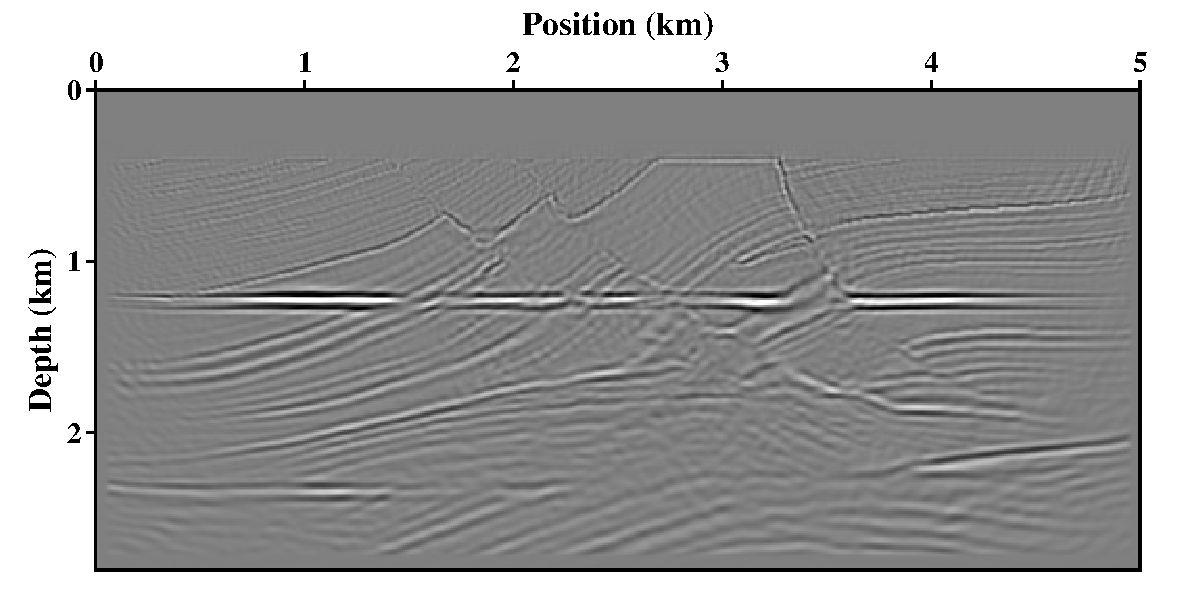
\includegraphics[width=0.5\textwidth]{Figure/chapter04/Marmousi/reflection/RTMvpdecomp.pdf}}
   \subfloat[]{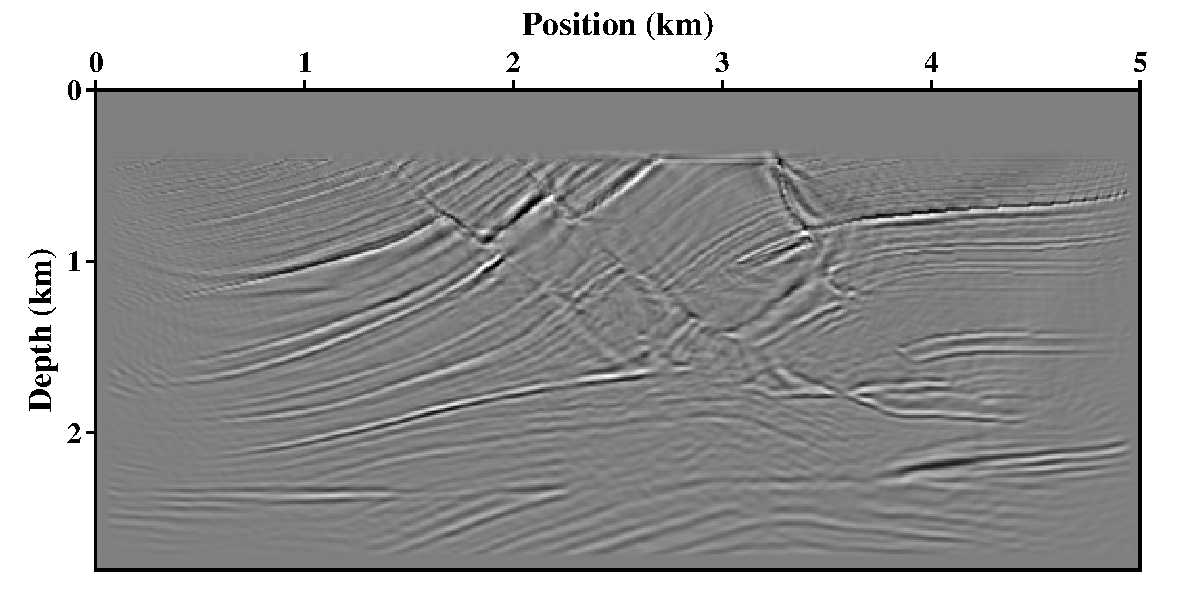
\includegraphics[width=0.5\textwidth]{Figure/chapter04/Marmousi/reflection/RTMvsdecomp.pdf}}\\
   \subfloat[]{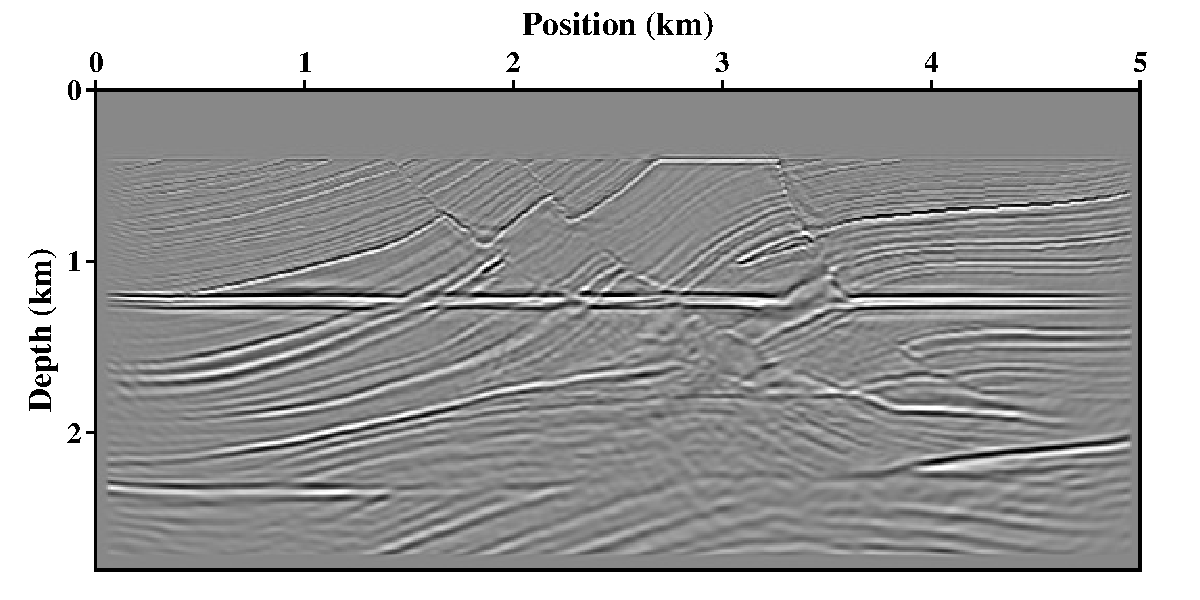
\includegraphics[width=0.5\textwidth]{Figure/chapter04/Marmousi/reflection/vpdecomp.pdf}}
   \subfloat[]{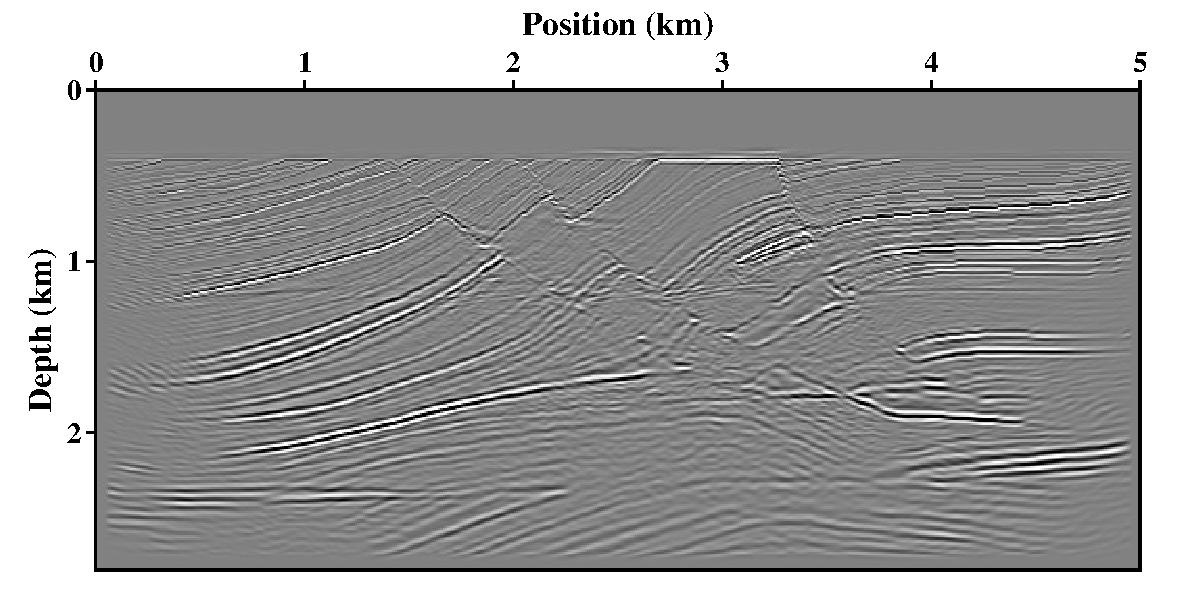
\includegraphics[width=0.5\textwidth]{Figure/chapter04/Marmousi/reflection/vsdecomp.pdf}}
   \caption{散射数据模式解耦ERTM与E-LSRTM结果。左侧为$V_p$,右侧为$V_s$。第一行为ERTM结果,第二行为E-LSRTM结果}
   \label{fig:LSRTM_1_refl}
\end{figure}

在引入模式解耦的梯度之后,可以看到ERTM结果中$\delta
V_s$的脚印已经被压制,在经过E-LSRTM之后,成像分辨率得到了提高,同时深部区域的能量也经过补偿获得了更好的均衡。
从结果上看Born数据要比散射数据的反演效果好,这是因为,第一,Born数据的正演与反演过程完全匹配;
第二,散射数据中存在多次散射效应,这导致深部的成像与反演质量较差。但是可以看到采用模式解耦的梯度能够在E-LSRTM基础上进一步压制参数耦合效应。
\begin{figure}[!htb]
   \centering
   \subfloat[]{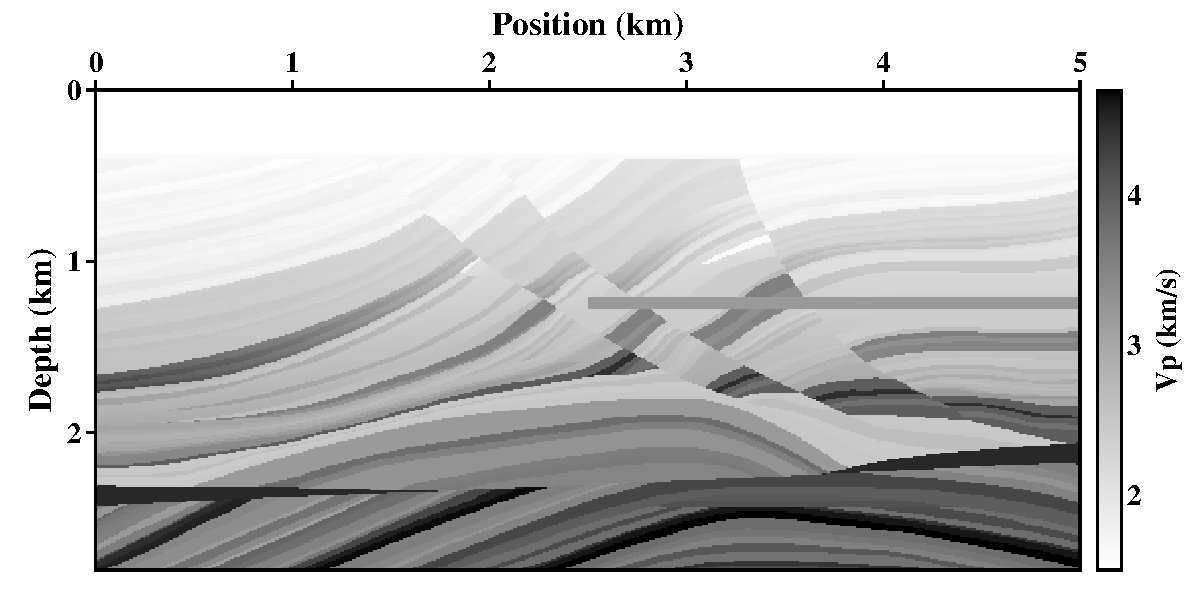
\includegraphics[width=0.5\textwidth]{Figure/chapter04/Marmousi/Vsborn/vp.pdf}}
   \subfloat[]{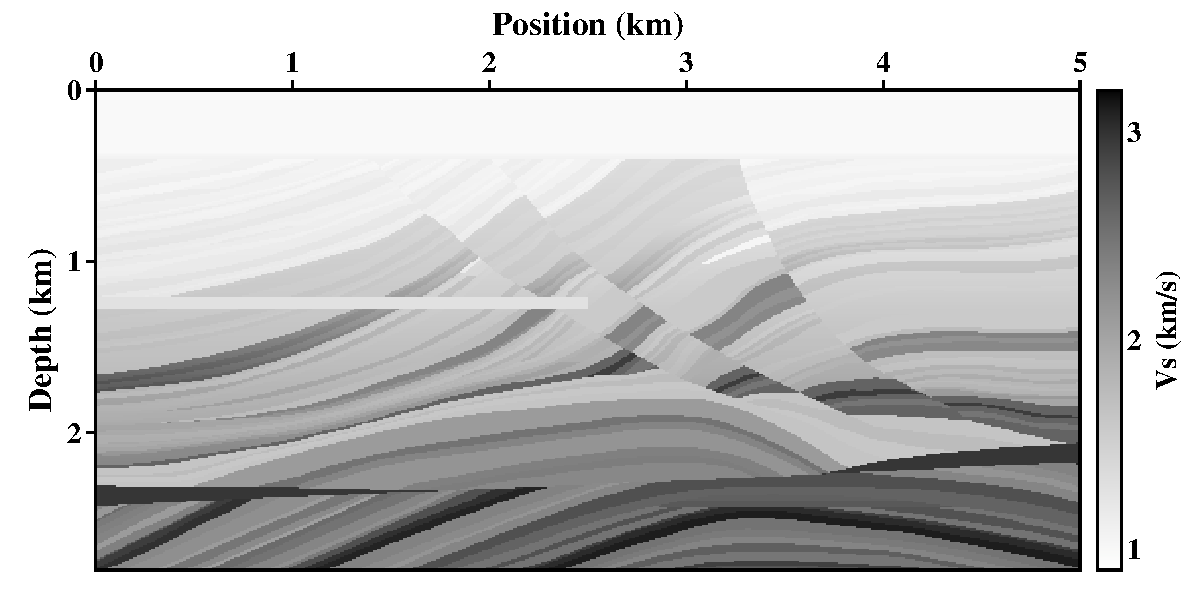
\includegraphics[width=0.5\textwidth]{Figure/chapter04/Marmousi/Vsborn/vs.pdf}}\\
   \subfloat[]{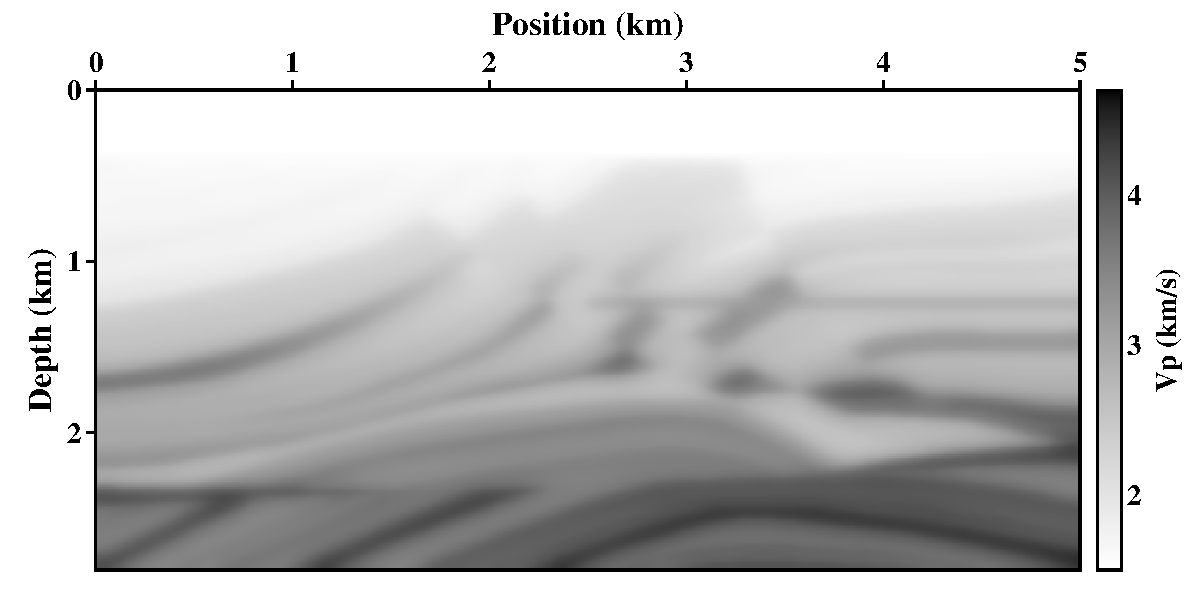
\includegraphics[width=0.5\textwidth]{Figure/chapter04/Marmousi/Vsborn/vpsmooth.pdf}}
   \subfloat[]{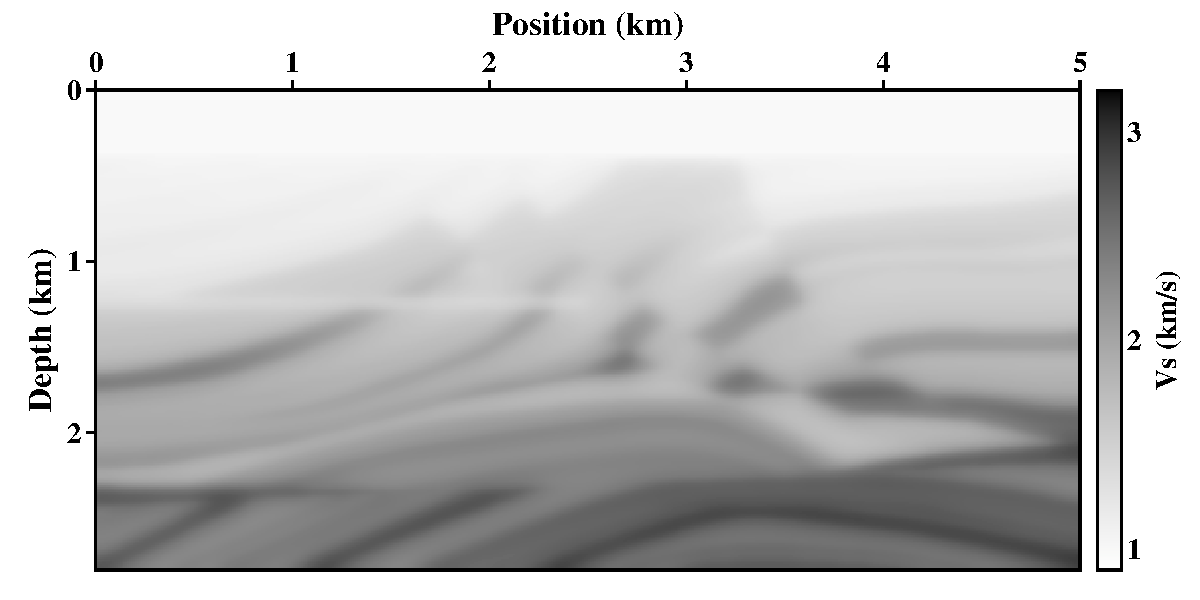
\includegraphics[width=0.5\textwidth]{Figure/chapter04/Marmousi/Vsborn/vssmooth.pdf}}
   \caption{Marmousi真实模型与偏移模型。}
   \label{fig:TrueAndInitial_2}
\end{figure}

\begin{figure}[!htb]
   \centering
   \subfloat[]{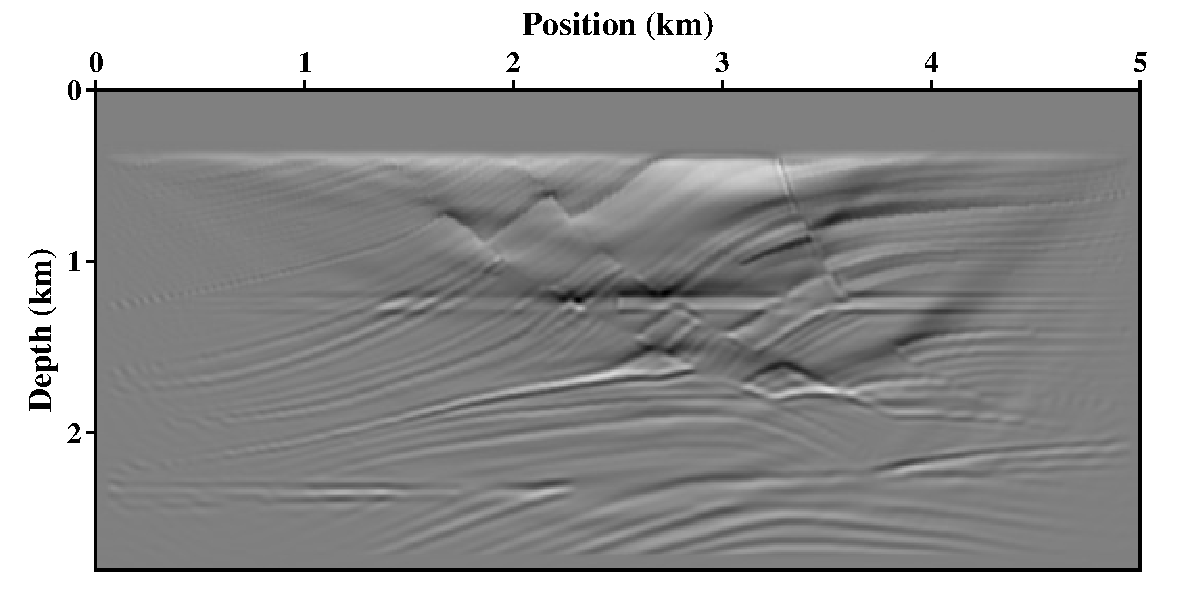
\includegraphics[width=0.5\textwidth]{Figure/chapter04/Marmousi/Vsborn/RTMvpnodecomp.pdf}}
   \subfloat[]{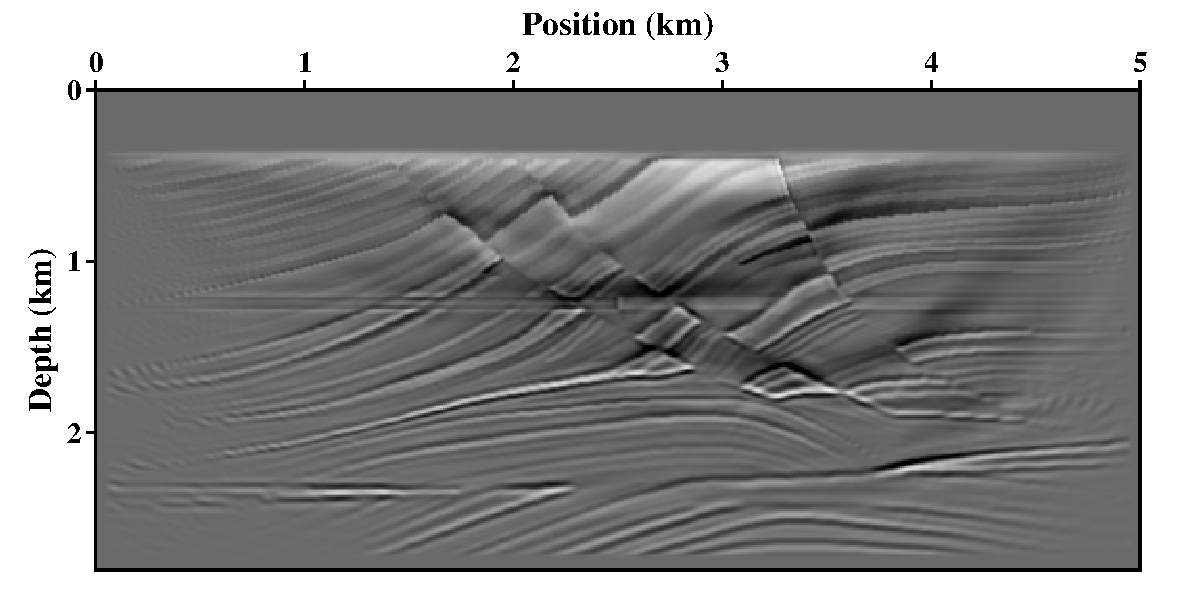
\includegraphics[width=0.5\textwidth]{Figure/chapter04/Marmousi/Vsborn/RTMvsnodecomp.pdf}}\\
   \subfloat[]{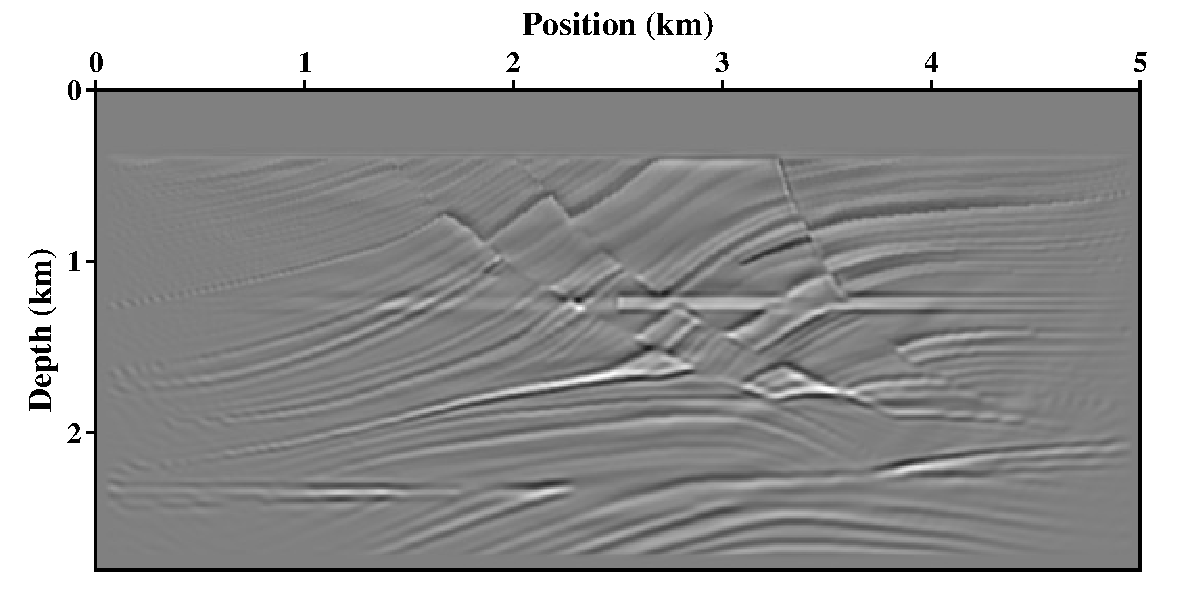
\includegraphics[width=0.5\textwidth]{Figure/chapter04/Marmousi/Vsborn/vpnodecomp.pdf}}
   \subfloat[]{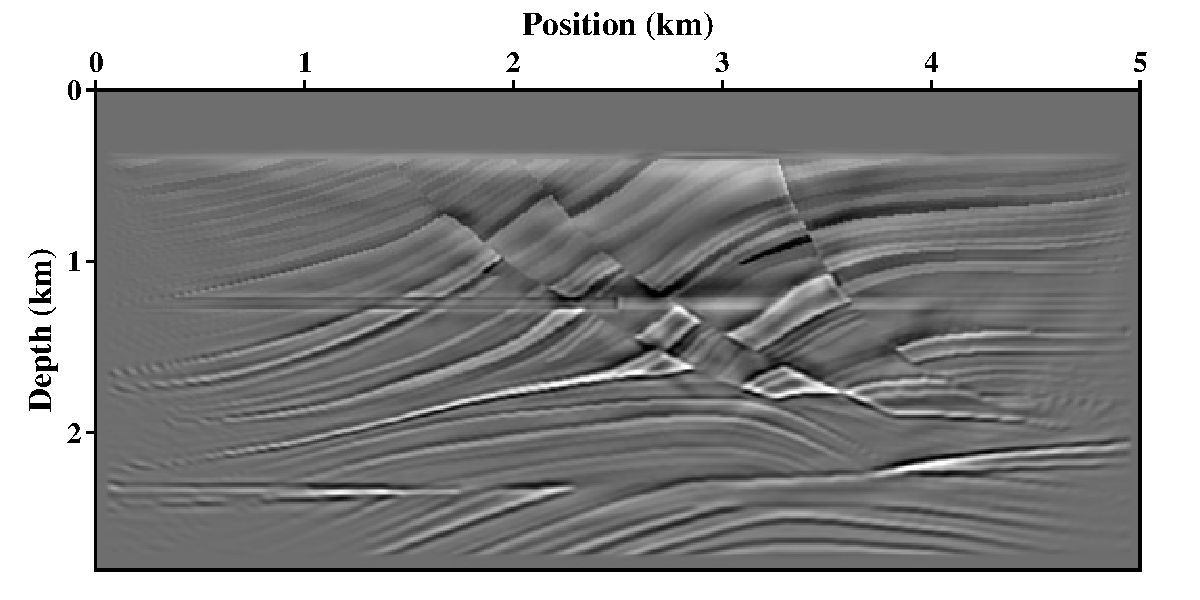
\includegraphics[width=0.5\textwidth]{Figure/chapter04/Marmousi/Vsborn/vsnodecomp.pdf}}
   \caption{Born数据常规ERTM与E-LSRTM结果,左侧为$V_p$,右侧为$V_s$。第一行为ERTM结果,第二行为E-LSRTM结果}
   \label{fig:nodecomp_2}
\end{figure}
\begin{figure}[!htb]
   \centering
   \subfloat[]{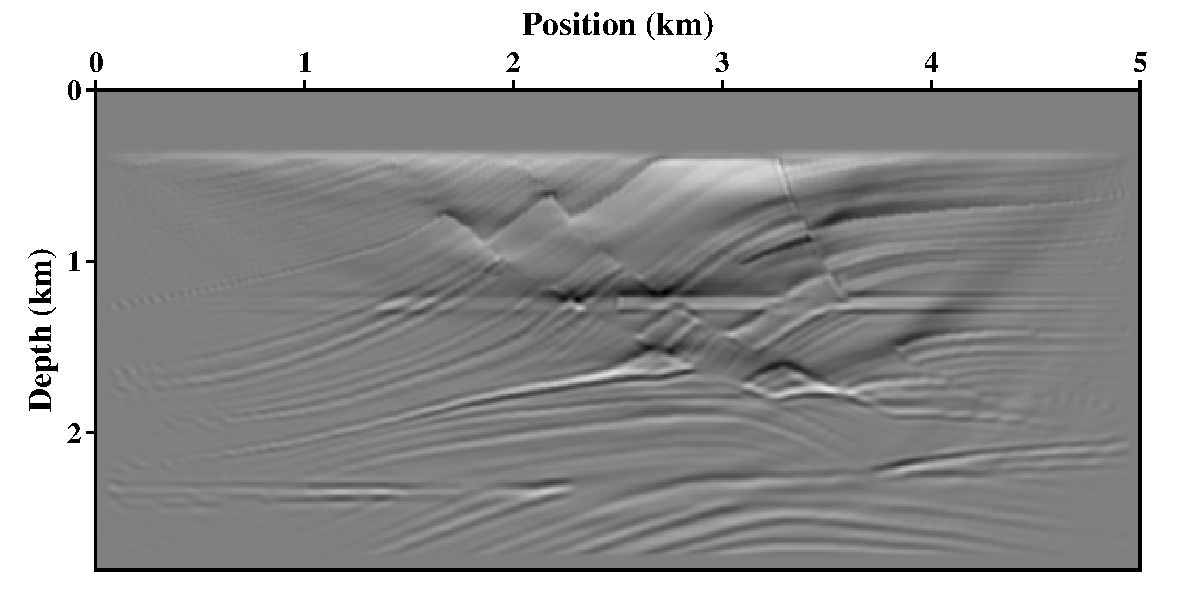
\includegraphics[width=0.5\textwidth]{Figure/chapter04/Marmousi/Vsborn/RTMvpdecomp.pdf}}
   \subfloat[]{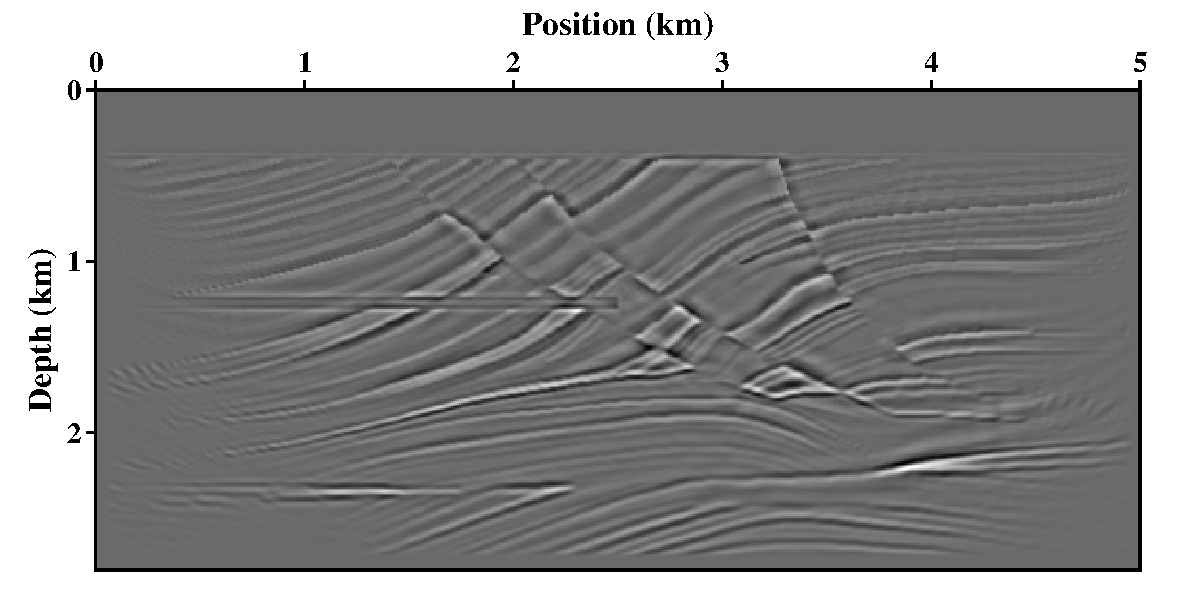
\includegraphics[width=0.5\textwidth]{Figure/chapter04/Marmousi/Vsborn/RTMvsdecomp.pdf}}\\
   \subfloat[]{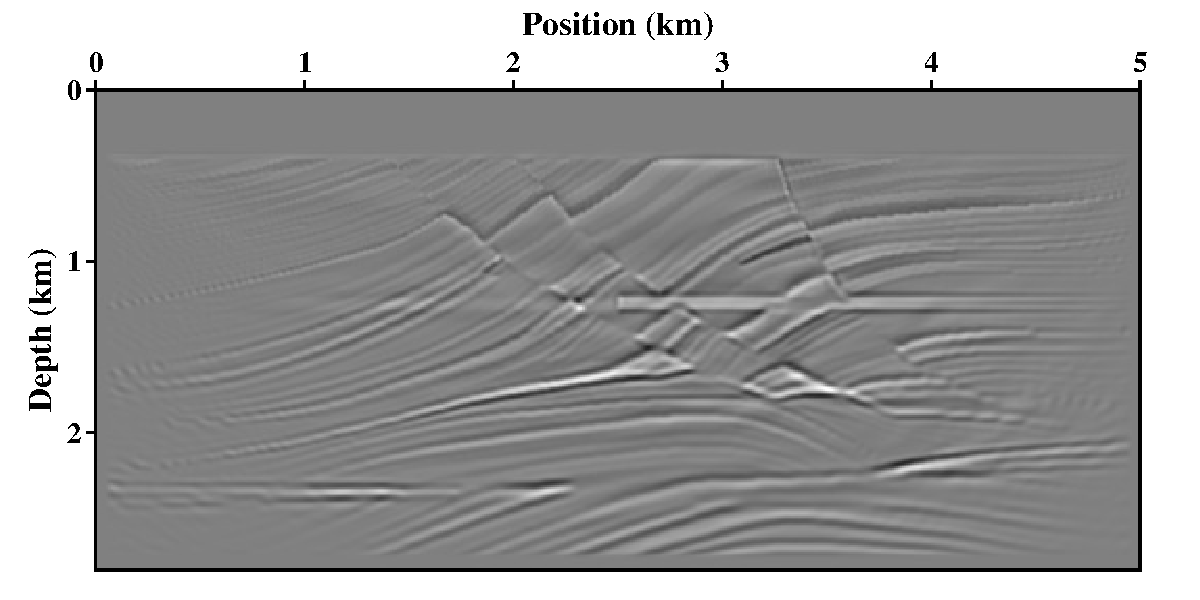
\includegraphics[width=0.5\textwidth]{Figure/chapter04/Marmousi/Vsborn/vpdecomp.pdf}}
   \subfloat[]{\includegraphics[width=0.5\textwidth]{Figure/chapter04/Marmousi/Vsborn/vsdecomp.pdf}}
   \caption{Born数据模式解耦ERTM与E-LSRTM结果,左侧为$V_p$,右侧为$V_s$。第一行为ERTM结果,第二行为E-LSRTM结果}
   \label{fig:decomp_2}
\end{figure}
第二个实验中,为了进一步突出参数耦合效应,我们在两个参数模型中分别加入速度异常结构(图\ref{fig:TrueAndInitial_2})。
这样参数耦合会在两个参数产生比较严重的相互干扰,这在实际数据是很容易遇到的情况。
此时如果考虑同时反演的策略1,参数耦合会导致
E-LSRTM的非线性程度增高。Born数据的常规E-LSRTM成像结果中,$\delta
V_s$甚至还存在低频噪音,一个可能的原因就是$\delta V_s$中右侧受到参数耦合的干扰,导致P波残差没有或者错误的匹配造成的。
而加入模式解耦的梯度之后,不论ERTM还是E-LSRTM的结果都消除了$\delta
V_s$中的参数耦合,但是$\delta
V_p$中仍然存在部分的耦合脚印。这一部分脚印是由于$\delta
V_s$的反演没有完全收敛到真值,导致数据中总有来自$\delta V_s$的残余P波在$\delta
V_p$中成像。这部分假象很难被完全消除掉,这就需要考虑策略2来进行反演。并且在反射数据中,正反演过程并不完全匹配,
所以这种假象在同时反演中更难以被消除。我们将在反射数据实验中观察策略2的有效性。

\begin{figure}[!htb]
   \centering
   \subfloat[]{\includegraphics[width=0.5\textwidth]{Figure/chapter04/Marmousi/Vsreflection/RTMvpnodecomp.pdf}}
   \subfloat[]{\includegraphics[width=0.5\textwidth]{Figure/chapter04/Marmousi/Vsreflection/RTMvsnodecomp.pdf}}\\
   \subfloat[]{\includegraphics[width=0.5\textwidth]{Figure/chapter04/Marmousi/Vsreflection/vpnodecomp.pdf}}
   \subfloat[]{\includegraphics[width=0.5\textwidth]{Figure/chapter04/Marmousi/Vsreflection/vsnodecomp.pdf}}
   \caption{反射数据常规ERTM与E-LSRTM结果,左侧为$V_p$,右侧为$V_s$。第一行为ERTM结果,第二行为E-LSRTM结果}
   \label{fig:nodecomp_2_refl}
\end{figure}
\begin{figure}[!htb]
   \centering
   \subfloat[]{\includegraphics[width=0.5\textwidth]{Figure/chapter04/Marmousi/Vsreflection/RTMvpdecomp.pdf}}
   \subfloat[]{\includegraphics[width=0.5\textwidth]{Figure/chapter04/Marmousi/Vsreflection/RTMvsdecomp.pdf}}\\
   \subfloat[]{\includegraphics[width=0.5\textwidth]{Figure/chapter04/Marmousi/Vsreflection/vpdecomp.pdf}}
   \subfloat[]{\includegraphics[width=0.5\textwidth]{Figure/chapter04/Marmousi/Vsreflection/vsdecomp.pdf}}\\
   \caption{反射数据模式解耦ERTM与E-LSRTM结果,左侧为$V_p$,右侧为$V_s$。第一行为ERTM结果,第二行为E-LSRTM结果}
   \label{fig:decomp_2_refl}
\end{figure}
\begin{figure}[!htb]
   \centering
   \subfloat[]{\includegraphics[width=0.5\textwidth]{Figure/chapter04/Marmousi/Vsreflection/vpdecomp.pdf}}
   \subfloat[]{\includegraphics[width=0.5\textwidth]{Figure/chapter04/Marmousi/Vsreflection/firstvs2ndvpdecomp.pdf}}
   \caption{Sigbee2A model example. On the top are true models of 
   $V_p$ (a) and $V_s$ (b). On the bottom are initial models of $V_p$ (c) and $V_s$
   (d) linearly increasing with depth. }
   \label{fig:final_comparison_2}
\end{figure}
针对反射数据,同样将数据中的直达波进行切除,
首先进行双参数同时反演。其常规ERTM与E-LSRTM的结果与前述实验结果类似,E-LSRTM可以改善成像质量,提高分辨率,
并部分压制参数耦合效应。在采用解耦预条件的梯度之后,ERTM以及E-LSRTM结果中$\delta
V_s$的假象有所改善,但是$\delta
V_p$中的假象仍然存在。此后我们又采用策略2来进行反演,
先采用解耦预条件的方式反演好$\delta V_s$,其次固定反演好的$\delta V_s$来反演$\delta
V_p$。由于第一阶段中只匹配S波残差,因此反演结果基本与图\ref{fig:decomp_2}c中结果一致,这里由于篇幅限制就不再展示。
而采用两步法反演的$\delta
V_p$如图\ref{fig:final_comparison_2}b所示,可以看到左侧速度结构异常区域的干扰被进一步压制。但是由于$\delta V_s$反演并未完全消除其产生的P波残差,因此最后的反演结果中仍然存在少量的干扰。
\section{本章小结}
E-LSRTM可视为线性的EFWI过程,其同样会受到参数耦合的影响。虽然该过程中
可以提高成像分辨率并部分压制参数耦合,但是无法做到完全压制。模式解耦的预条件方式可以非常有效地压制$\delta
V_s$反演中来自$\delta V_p$的影响。
在$\delta V_p$受参数耦合影响较弱时,在模式解耦的帮助下进行双参数同时反演可以快速地获得$\delta
V_s$与$\delta V_p$。而在$\delta V_p$受参数耦合影响较强时,可以通过先反演$\delta V_s$后反演$\delta
V_p$来进一步压制$\delta V_p$中来自$\delta V_s$耦合效应干扰。

E-LSRTM过程中,由于Born数据与反射数据之间的差异,直接匹配反射数据会导致界面参数扰动的过估计,
而匹配剩余反射数据则可以更好地近似Born散射过程。此外,在模型复杂区域,反射数据中包含有多次散射效应,这些散射波会带来较多的干扰。
